\section{Funções de Engenharia}

Para cada função existente no projeto, seus \textit{inputs}, \textit{outputs} e definições do que se retornam estão definidos no que se segue, sendo alguns responsáveis por informações contidas no banco de dados local ou presente nas bibliotecas em utilização, enquanto outros são responsáveis por calcular parâmetros de projeto.

\subsection{Dimensionamento de Tubulações}

Tubulações são componentes por onde o fluido escoa, permitindo a transferência de matéria entre equipamentos, desde a entrada de matéria-prima até a saída de produtos. Seu correto dimensionamento é imprescindível para a segurança e a eficiência do processo.

O dimensionamento consiste em definir o diâmetro nominal e o \textit{schedule} capazes de conduzir as vazões dentro de faixas de velocidade e perda de carga economicamente ótimas. As grandezas envolvidas incluem vazão (mássica ou volumétrica), velocidade admissível, propriedades do fluido (massa específica, viscosidade), comprimento equivalente (devido a acessórios) e características do material (rugosidade, pressão de projeto).

Na prática, calcula-se um diâmetro a partir da vazão e velocidade alvo e seleciona-se o diâmetro comercial imediatamente superior disponível, verificando em seguida a perda de carga pelo método de Darcy–Weisbach e a integridade mecânica conforme normas aplicáveis. Temperatura e pressão afetam propriedades físicas do fluido e critérios de espessura da tubulação; adicionalmente, a topografia da planta e o número de acessórios elevam o comprimento equivalente total.

Subdimensionar uma linha implica grandes perdas de carga e custos energéticos; superdimensionar acarreta CAPEX elevado e pode gerar velocidades muito baixas (favorecendo sedimentação em linhas com sólidos). O embasamento teórico combina a equação de continuidade, correlações de atrito e seleção de materiais, apoiado no uso do diagrama de Moody \cite{white2018}.

\subsubsection{Diâmetro Calculado}

O diâmetro calculado é baseado na vazão e na velocidade média do fluido escoando em um duto circular, de acordo com a Equação \ref{eq:diametro_calc}:

\begin{equation}
D = \sqrt{\frac{4 \cdot Q}{\pi \cdot V}}
\label{eq:diametro_calc}
\end{equation}

Dos quais,
\begin{itemize}
    \item Q – Vazão volumétrica do fluido;
    \item V – Velocidade do fluido;
    \item D - Diâmetro hidráulico do duto circular.
\end{itemize}

Essa relação advém diretamente da equação da continuidade para escoamento em regime permanente \cite{white2018}. No código, a função \textit{get\_calculated\_diameter} presente na classe dos cálculos hidráulicos utiliza o controle de unidades via \textit{Pint} e retorna o resultado em milímetros, assegurando consistência dimensional.

\begin{figure}[H]
    \centering
    \caption{Código da função \textit{get\_calculated\_diameter()}}
    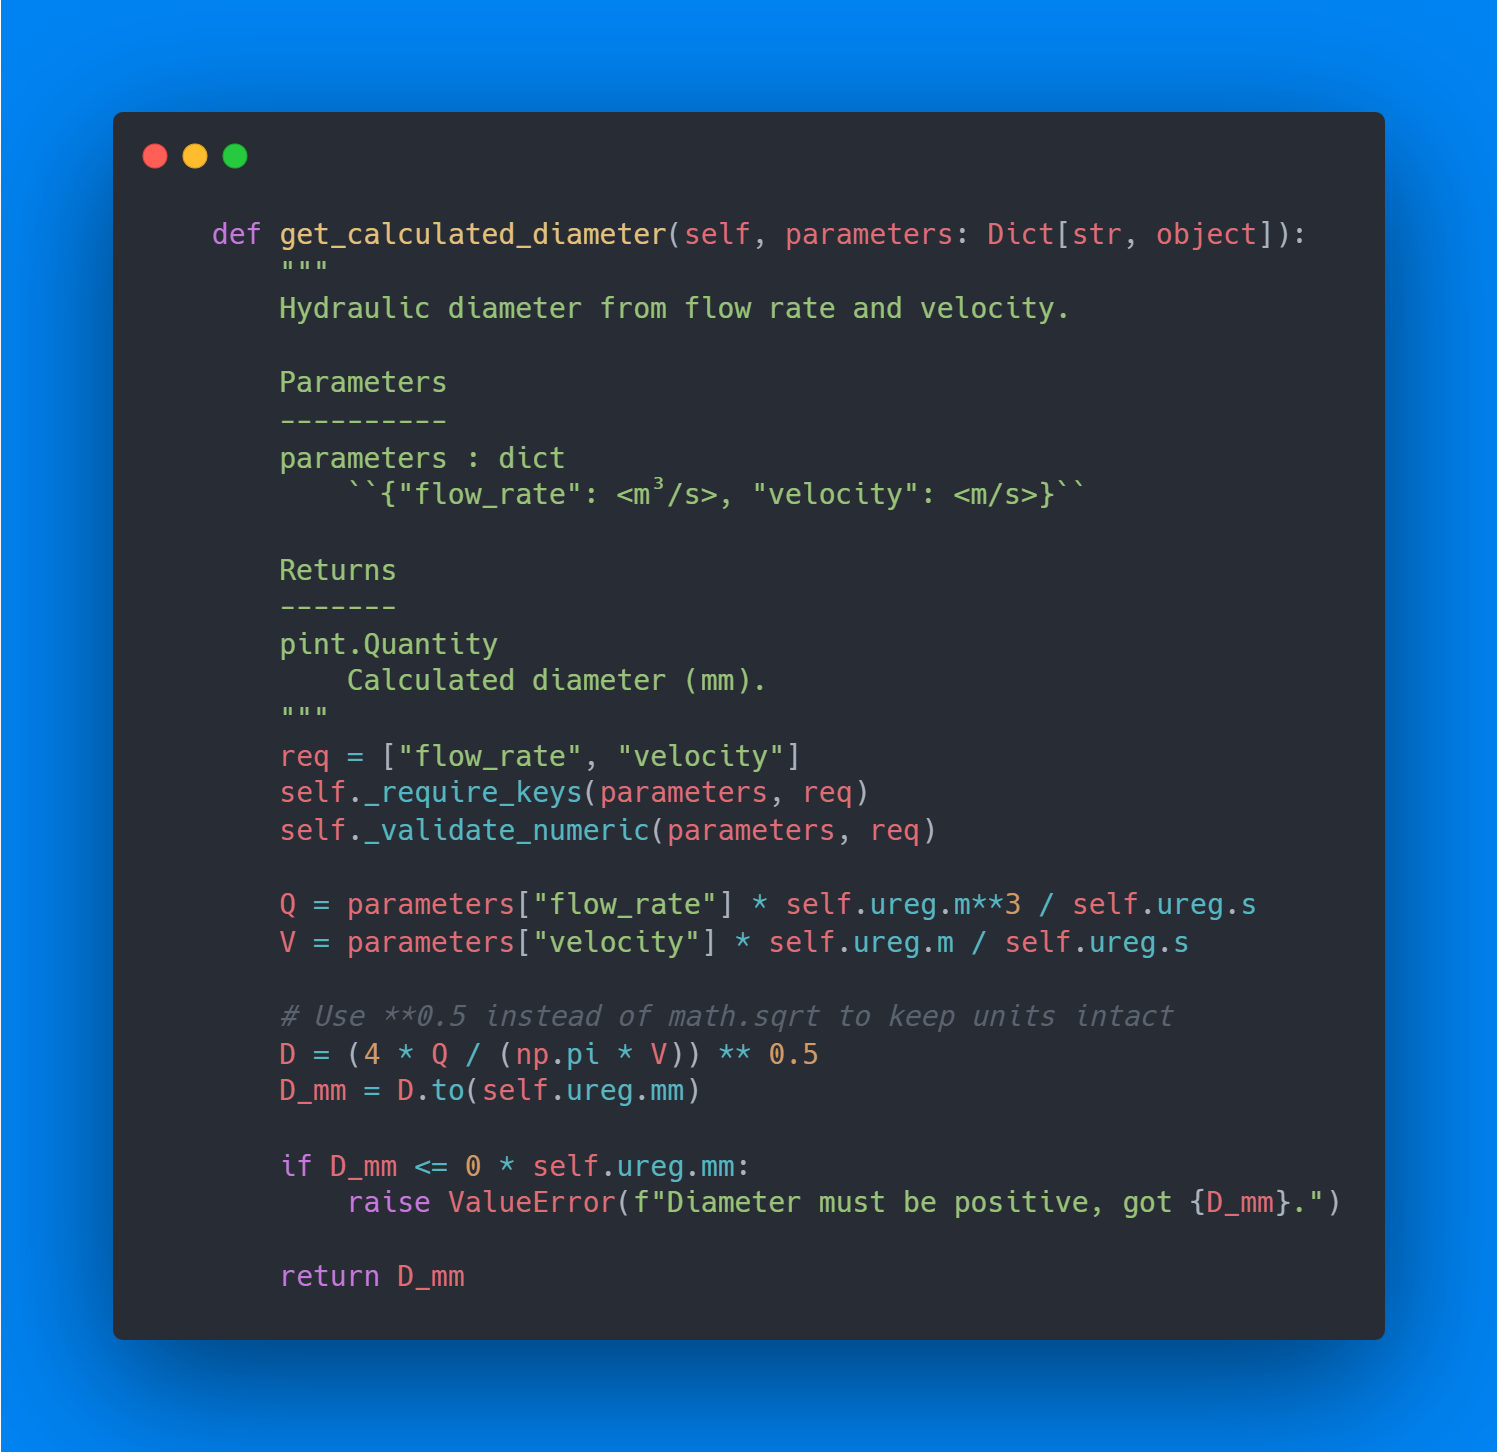
\includegraphics[width=\linewidth]{media/0d3b6479c2817c517ba7848c8aafdbe8.png}
    \fonte{Autoria própria.}
\end{figure}

\subsubsection{Diâmetro Real}

O diâmetro real corresponde ao diâmetro nominal da tubulação a ser utilizada. Fabricantes produzem tubos em geometrias padronizadas (padrões de espessura como SCH 10, SCH 40, SCH 80 etc.). Deve-se calcular inicialmente o diâmetro necessário pelo método anterior e então escolher, em tabela de catálogo, a tubulação comercial com diâmetro interno imediatamente superior, no material e \textit{schedule} desejados. Essa lógica é implementada na função \textit{get\_real\_diameter}, garantindo que o diâmetro selecionado comportará a vazão com velocidade dentro do admissível. Após a seleção, verifica-se a perda de carga resultante e, se necessário, itera-se para outro diâmetro.

\begin{figure}[H]
    \centering
    \caption{Código da função \textit{get\_real\_diameter()}}
    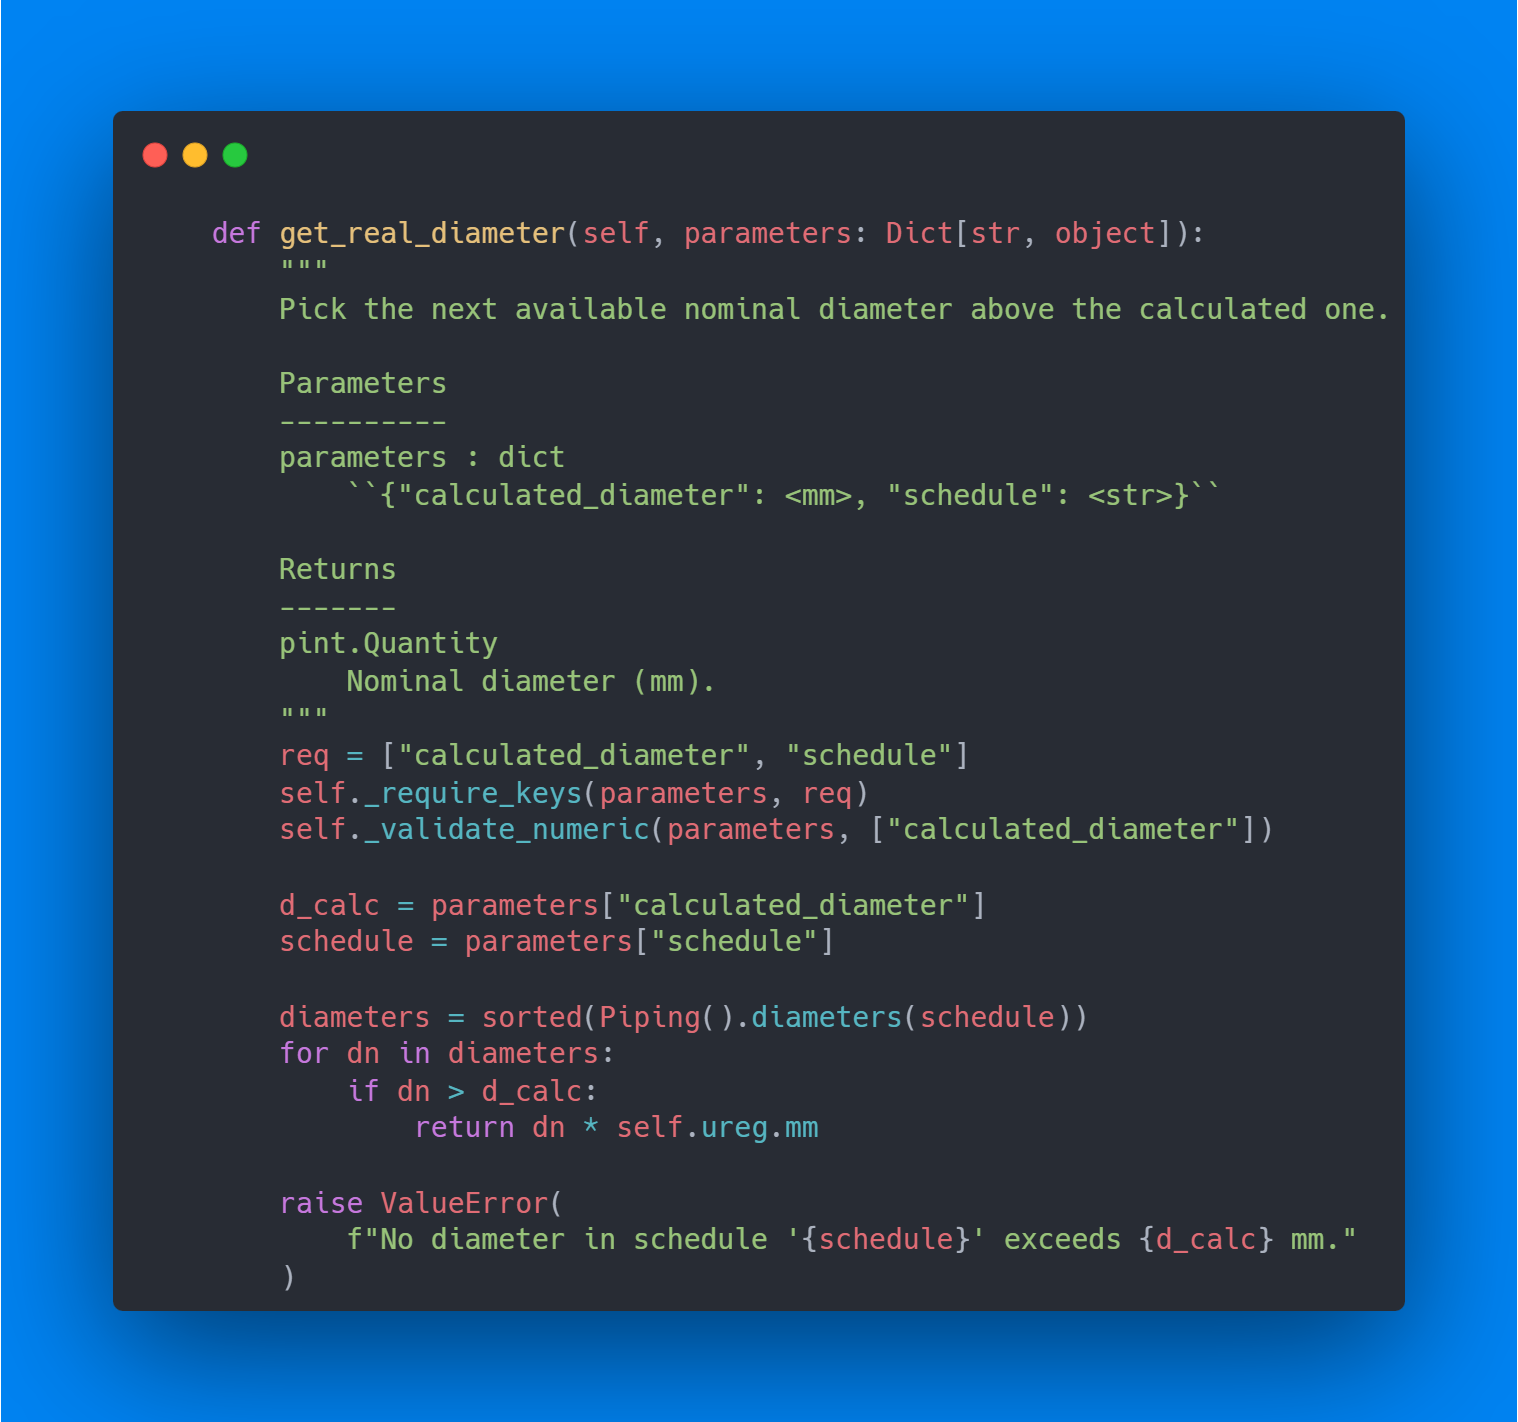
\includegraphics[width=\linewidth]{media/973bd6ac6b704ca56b2f3dbe6cece6bf.png}
    \fonte{Autoria própria.}
\end{figure}

\subsection{Reatores}

Reatores são equipamentos projetados para promover reações químicas, convertendo reagentes em produtos sob condições controladas de operação.

Modelos ideais como CSTR, PFR e batelada fornecem limites úteis para projeto e análise de desempenho. As variáveis centrais envolvidas no projeto de reatores incluem conversão dos reagentes, seletividade e rendimento (em caso de múltiplas reações), velocidade de reação, tempo de residência, volume do reator e condições de operação (temperatura, pressão). Industrialmente, o correto dimensionamento de reatores afeta diretamente a capacidade produtiva, a qualidade do produto e a segurança, especialmente no controle de remoção de calor em reações exotérmicas. A cinética química depende fortemente da temperatura (lei de Arrhenius) e da forma funcional da taxa de reação (ordem de reação, efeitos de inibição, presença de inertes, variação volumétrica em fase gasosa etc.). Erros na previsão de conversão ou no cálculo do volume reacional podem levar a baixa seletividade, formação de pontos quentes (hot spots) e riscos operacionais. A base teórica conjuga balanços de massa por componente com leis cinéticas apropriadas, integradas no espaço (PFR) ou no tempo de residência (CSTR), podendo incluir balanço de energia quando o regime térmico é relevante \cite{fogler2009,levenspiel2000}.

No escopo deste projeto, são considerados reatores isotérmicos e monofásicos (todos os reagentes e produtos em uma única fase, líquida ou gasosa). O código rejeita misturas de componentes em estados físicos diferentes, a fim de garantir a validade dos balanços e do fator de expansão volumétrica utilizado para o estado atual dos módulos de cálculo para reatores.

Algumas lógicas gerais se aplicam a todos os tipos de reatores implementados. Por exemplo, a determinação do reagente limitante, onde: identifica-se aquele reagente cuja razão entre a vazão molar de entrada e seu coeficiente estequiométrico é a menor dentre os reagentes presentes. Em termos de cálculo, percorrem-se os reagentes (coeficientes estequiométricos negativos), calculando conforme a Equação \ref{eq:razao_reagente}:
\begin{equation}
{razao}_{i} = \frac{N_{i 0}}{N_{u 0}}
\label{eq:razao_reagente}
\end{equation}, onde $N_{i 0}$ é a entrada molar do componente $i \  e$ $N_{u 0}$ seu coeficiente estequiométrico. O reagente com menor valor de ${razao}_{i}$ é o limitante \cite{felder2005}.

\begin{figure}[H]
    \centering
    \caption{Código da função \textit{determine\_limiting\_reagent()} – Parte 1/2}
    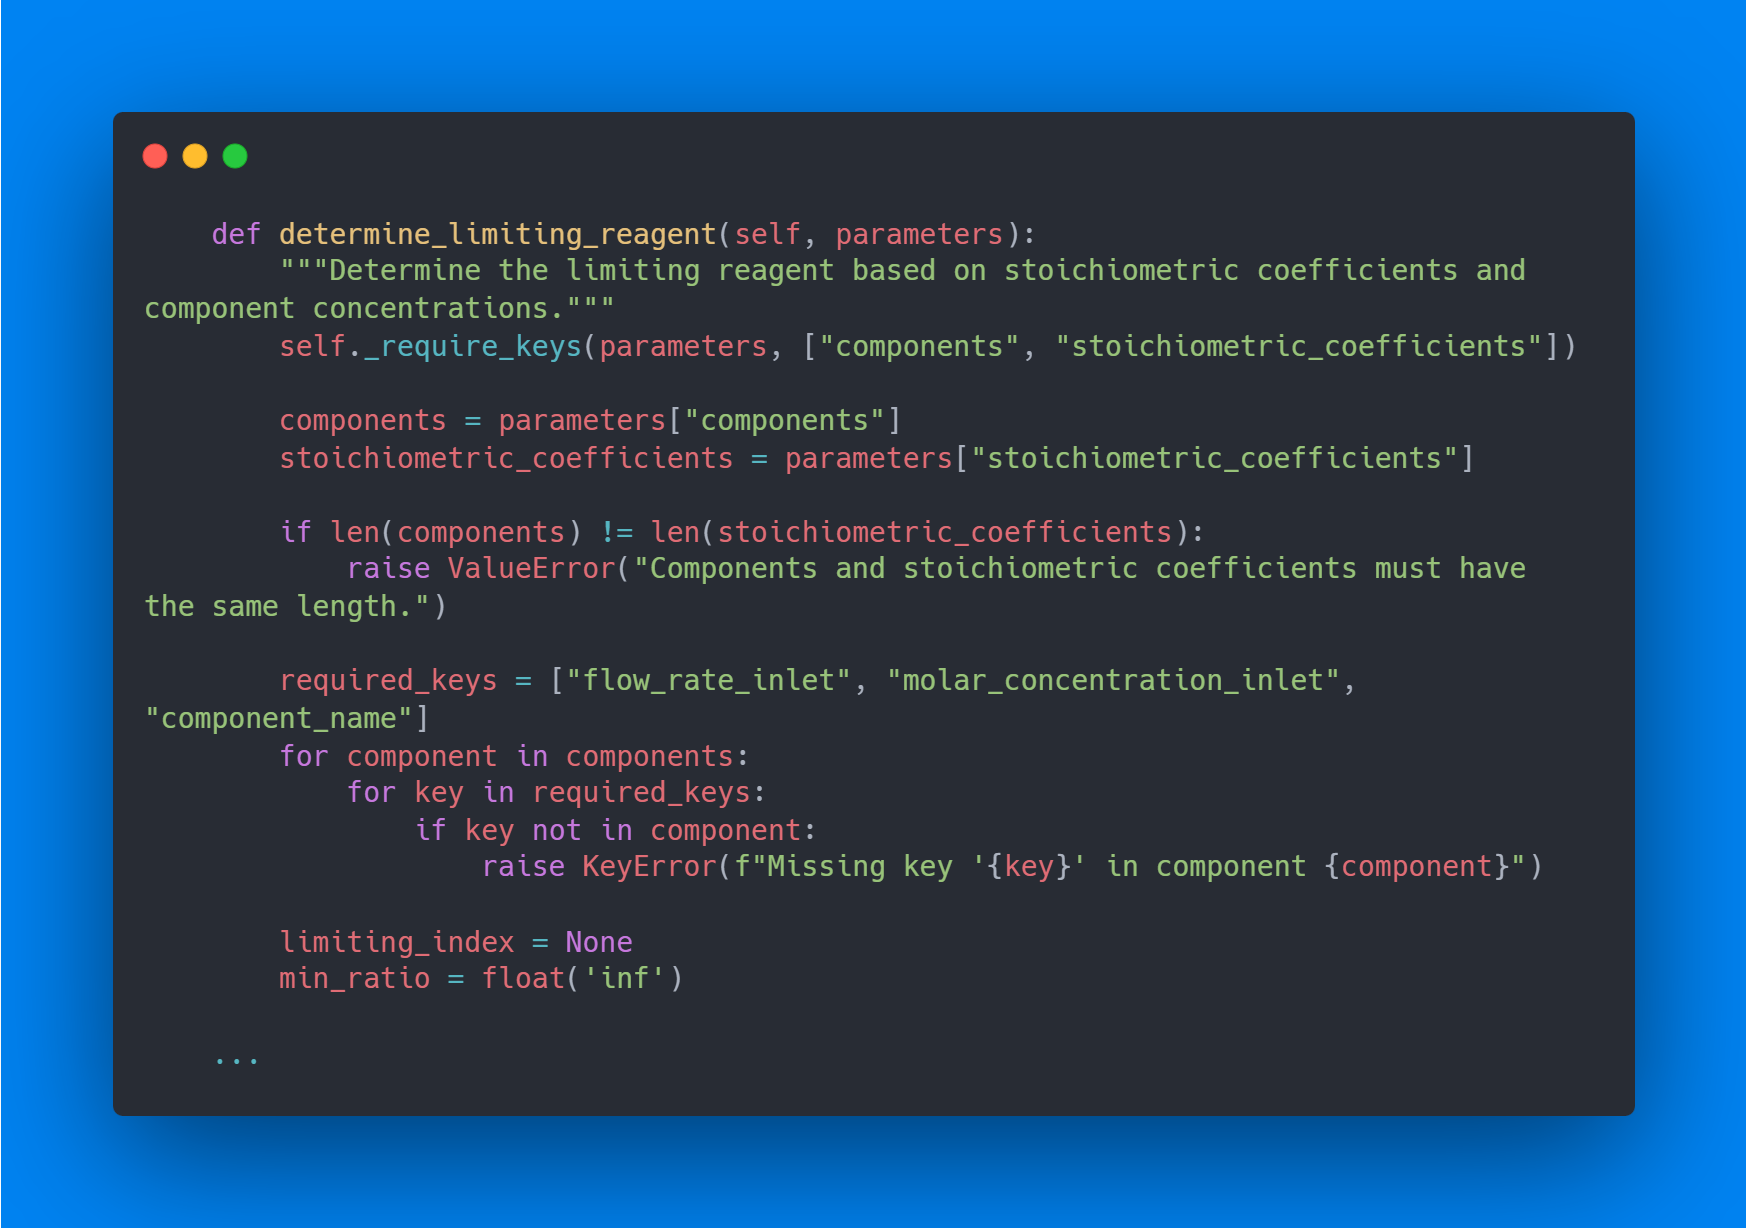
\includegraphics[width=\linewidth]{media/84378ecca8f6907d2498750ceacdb840.png}
    \fonte{Autoria própria.}
\end{figure}

\begin{figure}[H]
    \centering
    \caption{Código da função \textit{determine\_limiting\_reagent()} – Parte 2/2}
    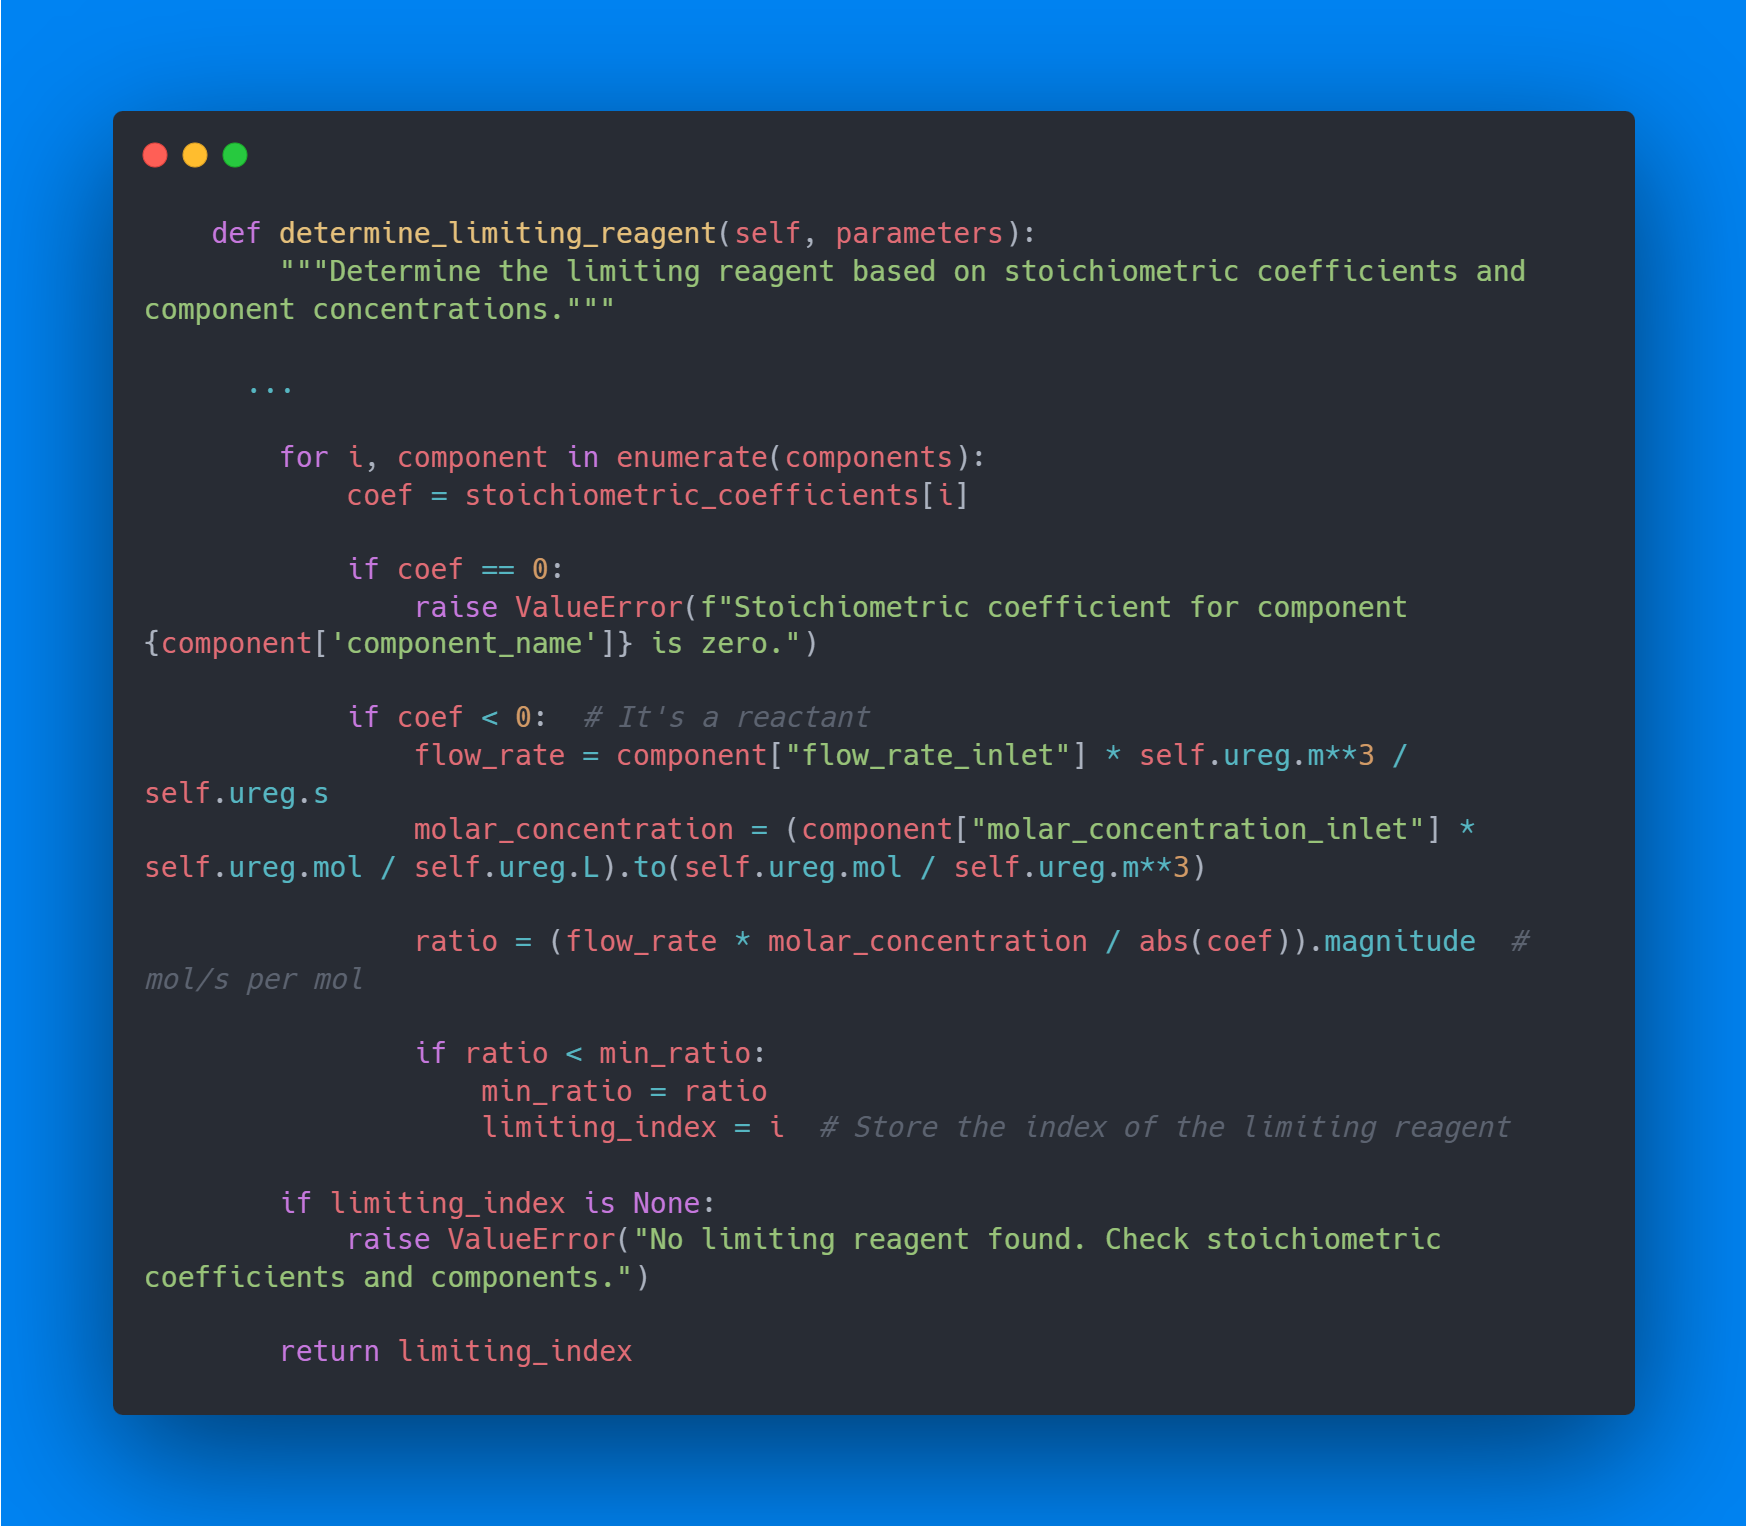
\includegraphics[width=\linewidth]{media/aec8d94ff156d2e683de34518553ec92.png}
    \fonte{Autoria própria.}
\end{figure}

A velocidade de reação é modelada, em geral, por uma lei de potência do tipo:

\begin{equation}
r = k \cdot \prod_{}^{} C_{i}^{n_{i}}
\label{eq:rate_law}
\end{equation}

Dos quais,
\begin{itemize}
    \item $C_{i}^{n_{i}}$ – Concentração de um reagente i elevado à sua ordem de velocidade em uma dada reação
    \item r – taxa de reação por volume;
    \item k constante de velocidade
\end{itemize}

\begin{figure}[H]
    \centering
    \caption{Código da função \textit{\_calculate\_concentration\_and\_rate()} – Trecho da velocidade da reação}
    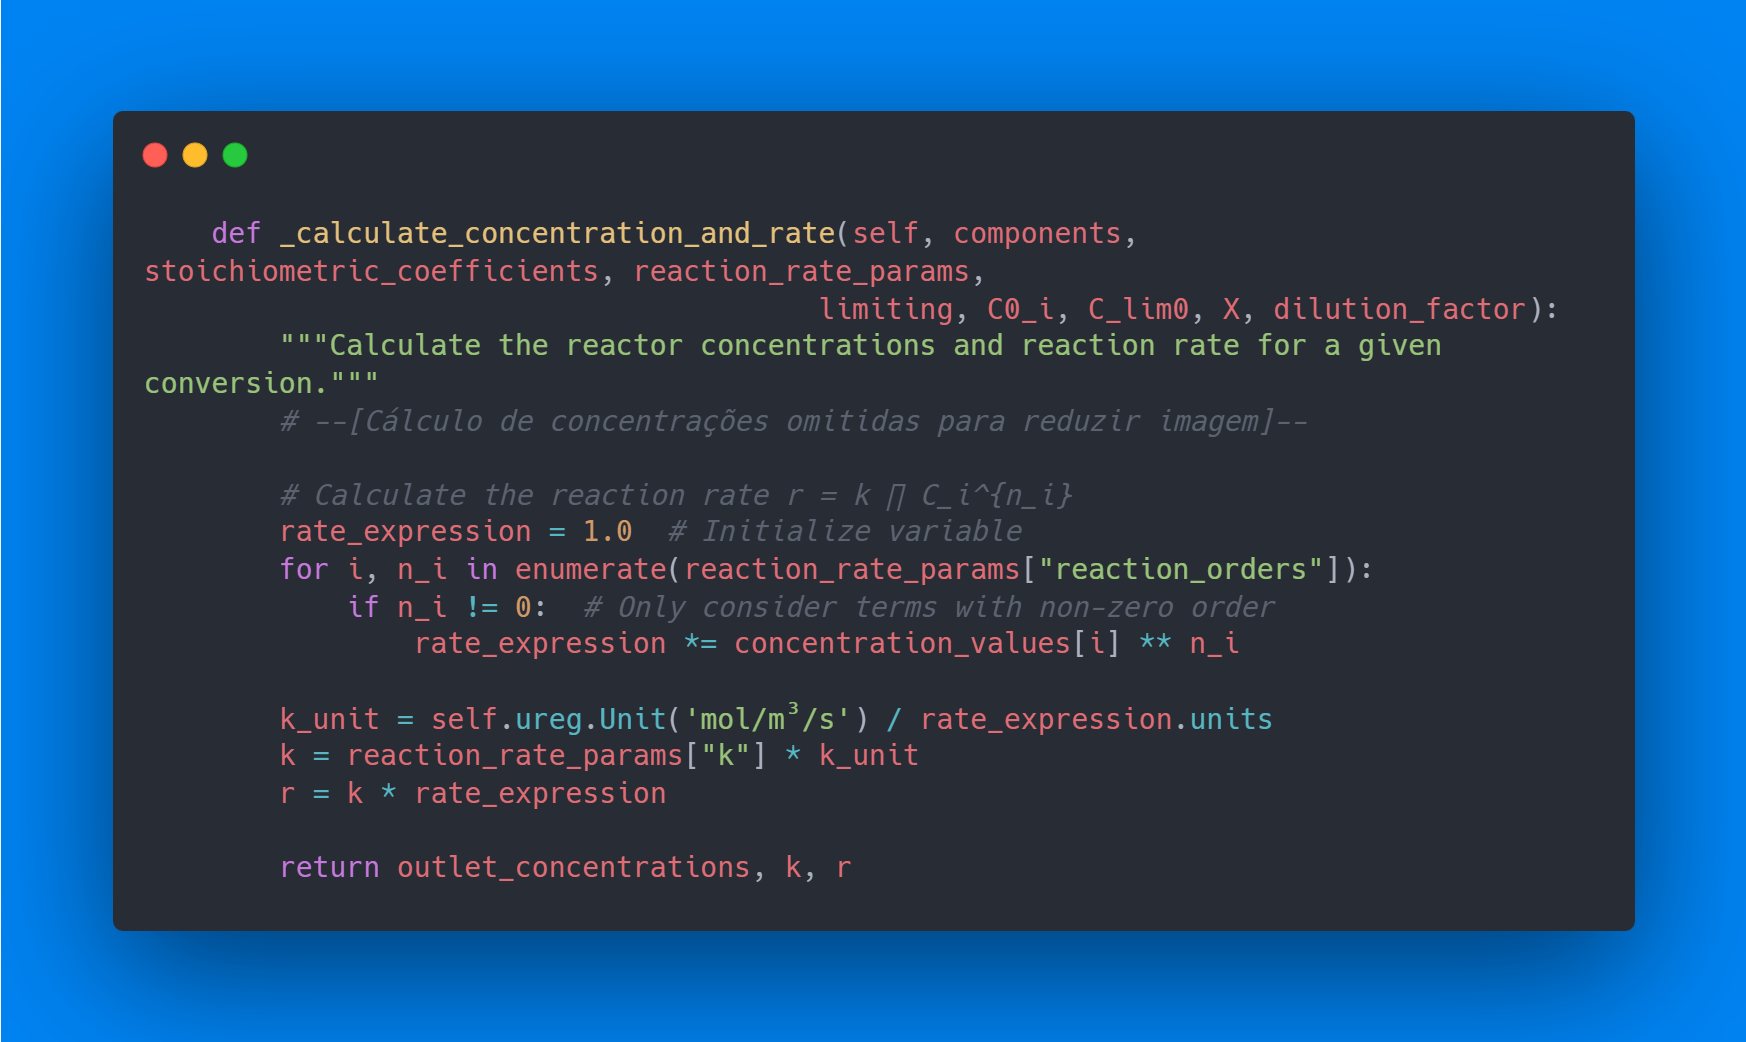
\includegraphics[width=\linewidth]{media/e431ad695f87a59080700db59c1a97a0.png}
    \fonte{Autoria própria.}
\end{figure}

A integração da cinética com a estequiometria é feita via conversão $X$ do reagente limitante. Os balanços estequiométricos relacionam as concentrações de saída de cada componente à conversão $X$. Para cada componente $i$ na reação, têm-se a seguinte relação geral, sendo o valor do mais ou menos positivo para formação (produtos), negativo para consumo (reagentes) e, claro, uma conversão igual a zero para inertes.

\begin{equation}
C_{i} = \frac{C_{i 0} \pm ( \frac{n_{i}}{n_{A}} \cdot C_{A} \cdot X )}{\varepsilon}
\label{eq:conc_stoich}
\end{equation}

Dos quais,
\begin{itemize}
    \item $C_{i}$ – Concentração do componente na saída
    \item $C_{i 0}$ – Concentração do componente na entrada
    \item $\varepsilon$ – Coeficiente de expansão volumétrico
    \item X – Conversão do reagente limitante
    \item $C_{A}$ – Concentração do reagente limitante
    \item $n_{i}$ – Coeficiente estequiométrico do componente
    \item $n_{A}$ – Coeficiente estequiométrico do reagente limitante
\end{itemize}

\begin{figure}[H]
    \centering
    \caption{Código da função \textit{\_calculate\_concentration\_and\_rate()} – Trecho da concentração dos componentes}
    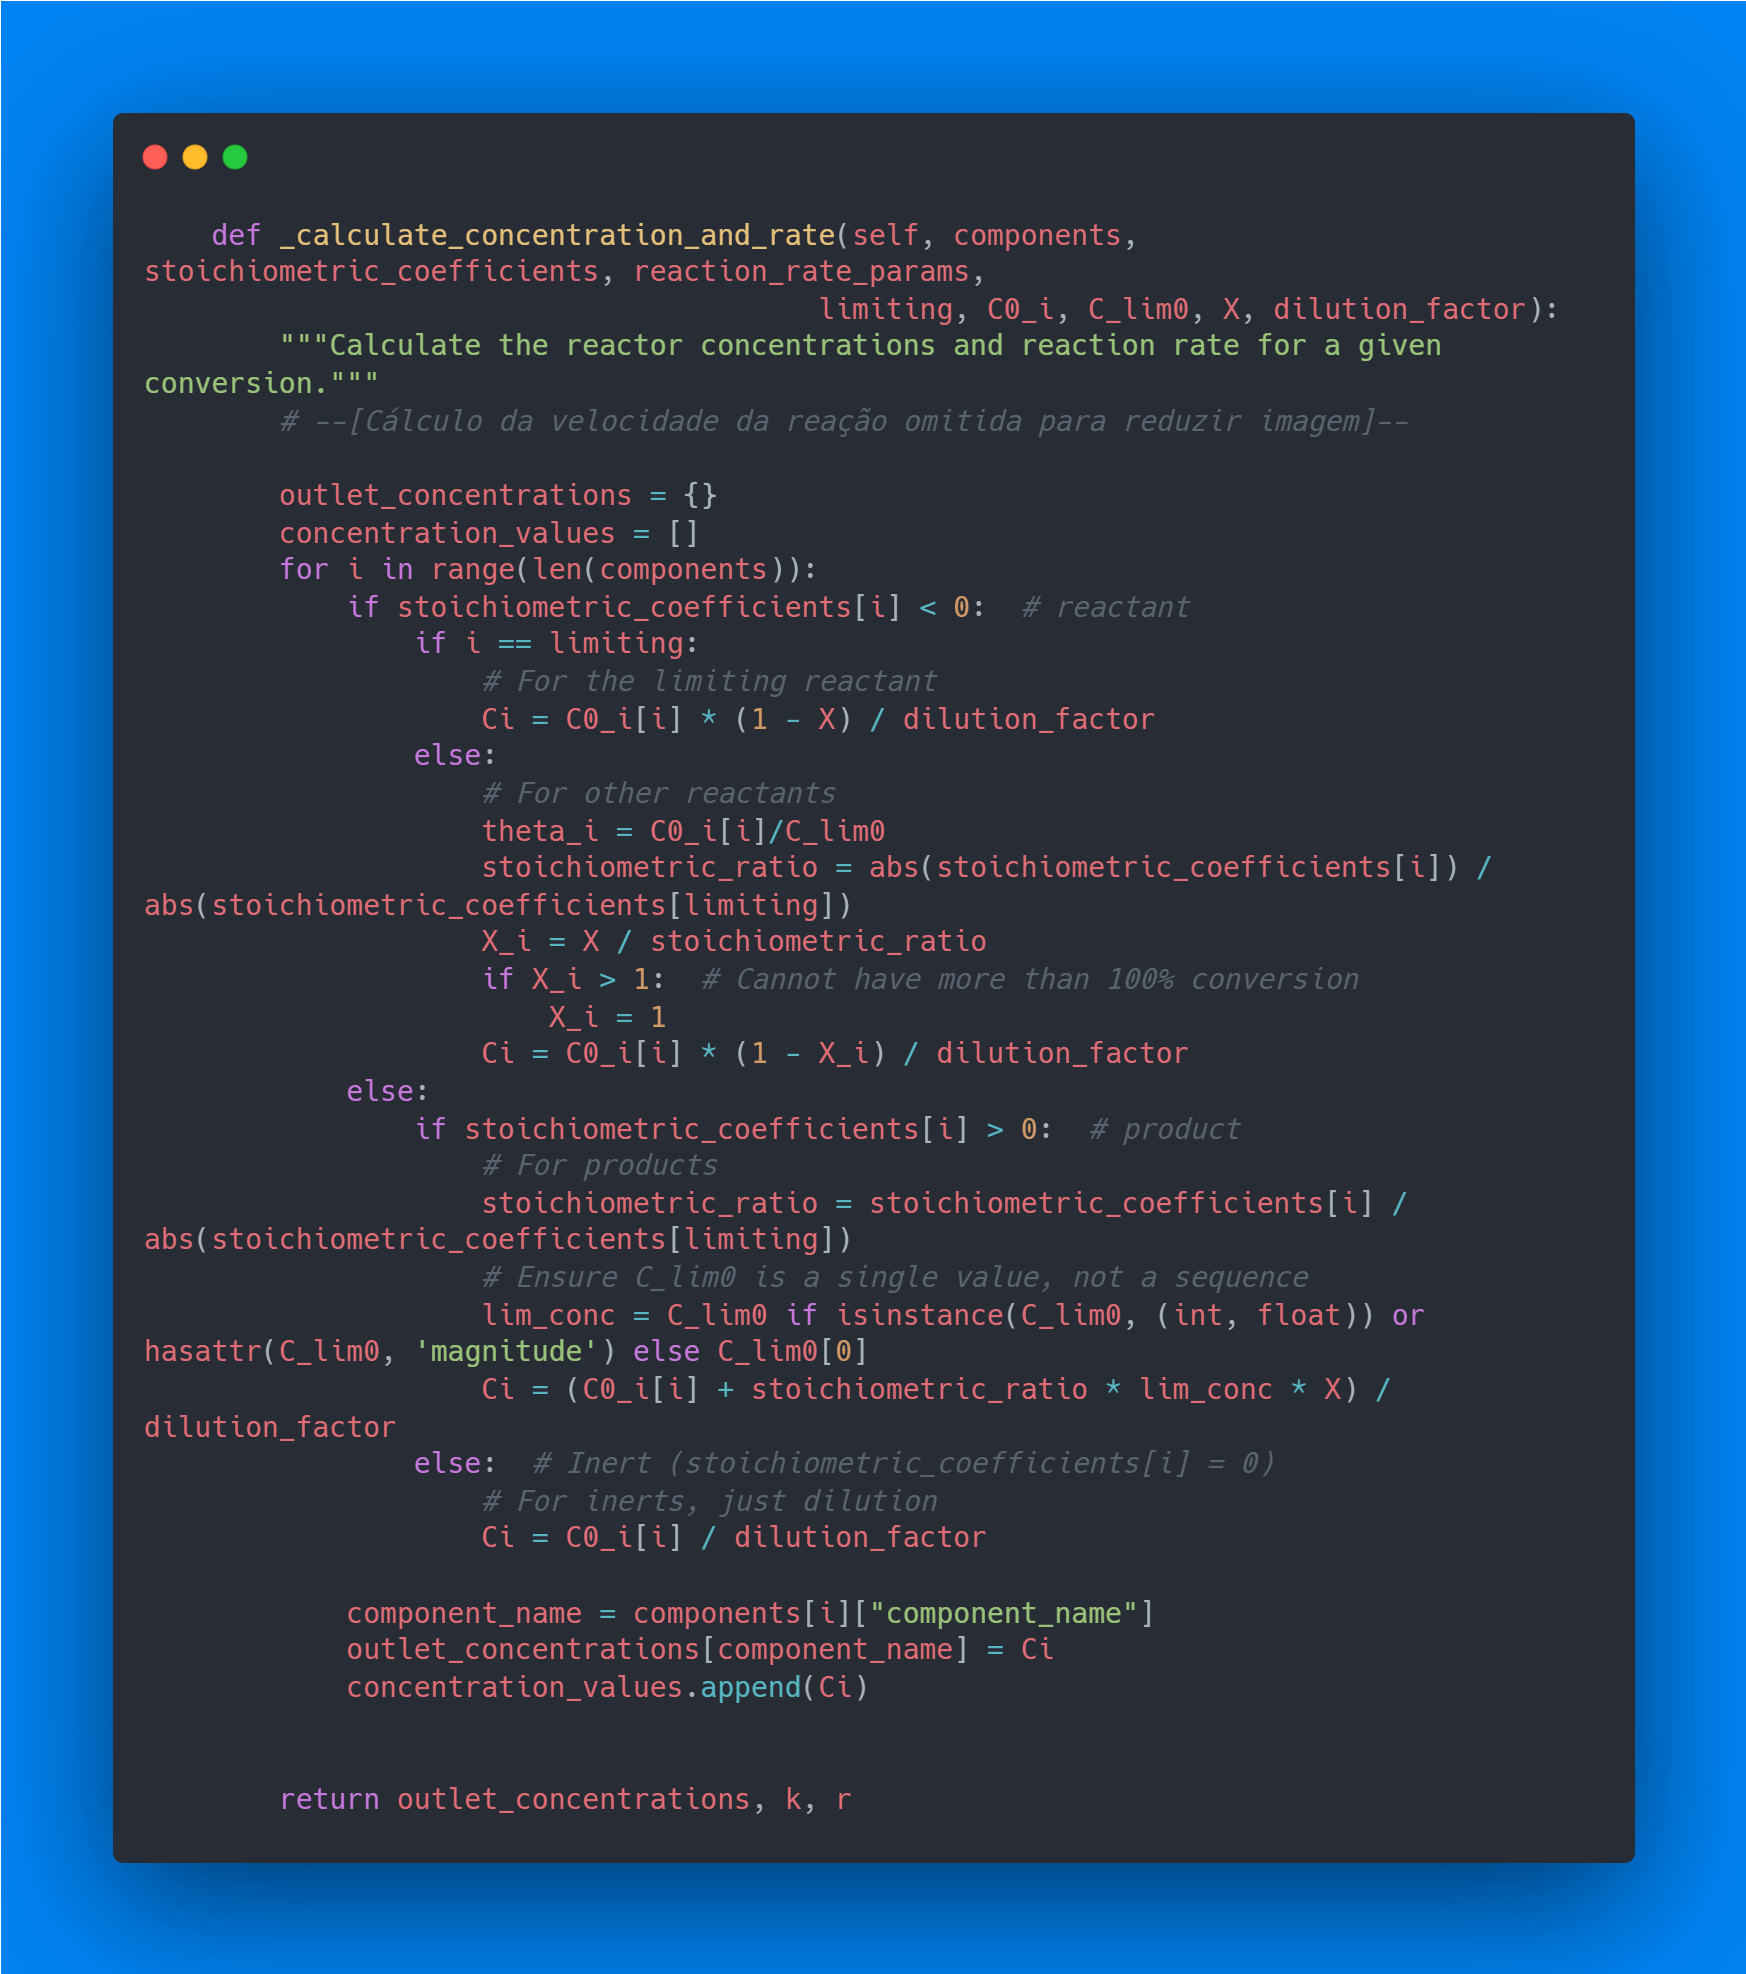
\includegraphics[width=\linewidth]{media/420d4eabc6222a8fb7b800c89334d0e4.png}
    \fonte{Autoria própria.}
\end{figure}

Para determinação do coeficiente de expansão volumétrico para reações gasosas, a Equação \ref{eq:epsilon_def} deve ser utilizada.

\begin{equation}
\varepsilon = y_{A0} \cdot \frac{\sum_{}^{} n_{P} - \sum_{}^{} n_{R}}{|n_{A}|}
\label{eq:epsilon_def}
\end{equation}

Dos quais,
\begin{itemize}
    \item $\sum_{}^{} n_{P}$ – Somatório dos coeficientes estequiométricos dos produtos gasosos;
    \item $\sum_{}^{} n_{R}$ – Somatório dos coeficientes estequiométricos dos reagentes gasosos;
    \item $y_{A0}$ – Fração molar do reagente limitante na alimentação;
    \item $n_{A}$ – Coeficiente estequiométrico do reagente limitante.
\end{itemize}

\begin{equation}
\varphi = ( 1 + \epsilon X ) \frac{P}{P_{0}} \frac{T_{0}}{T}
\label{eq:dilution_factor}
\end{equation}

\begin{figure}[H]
    \centering
    \caption{Código da função \textit{\_calculate\_dilution\_factor()}}
    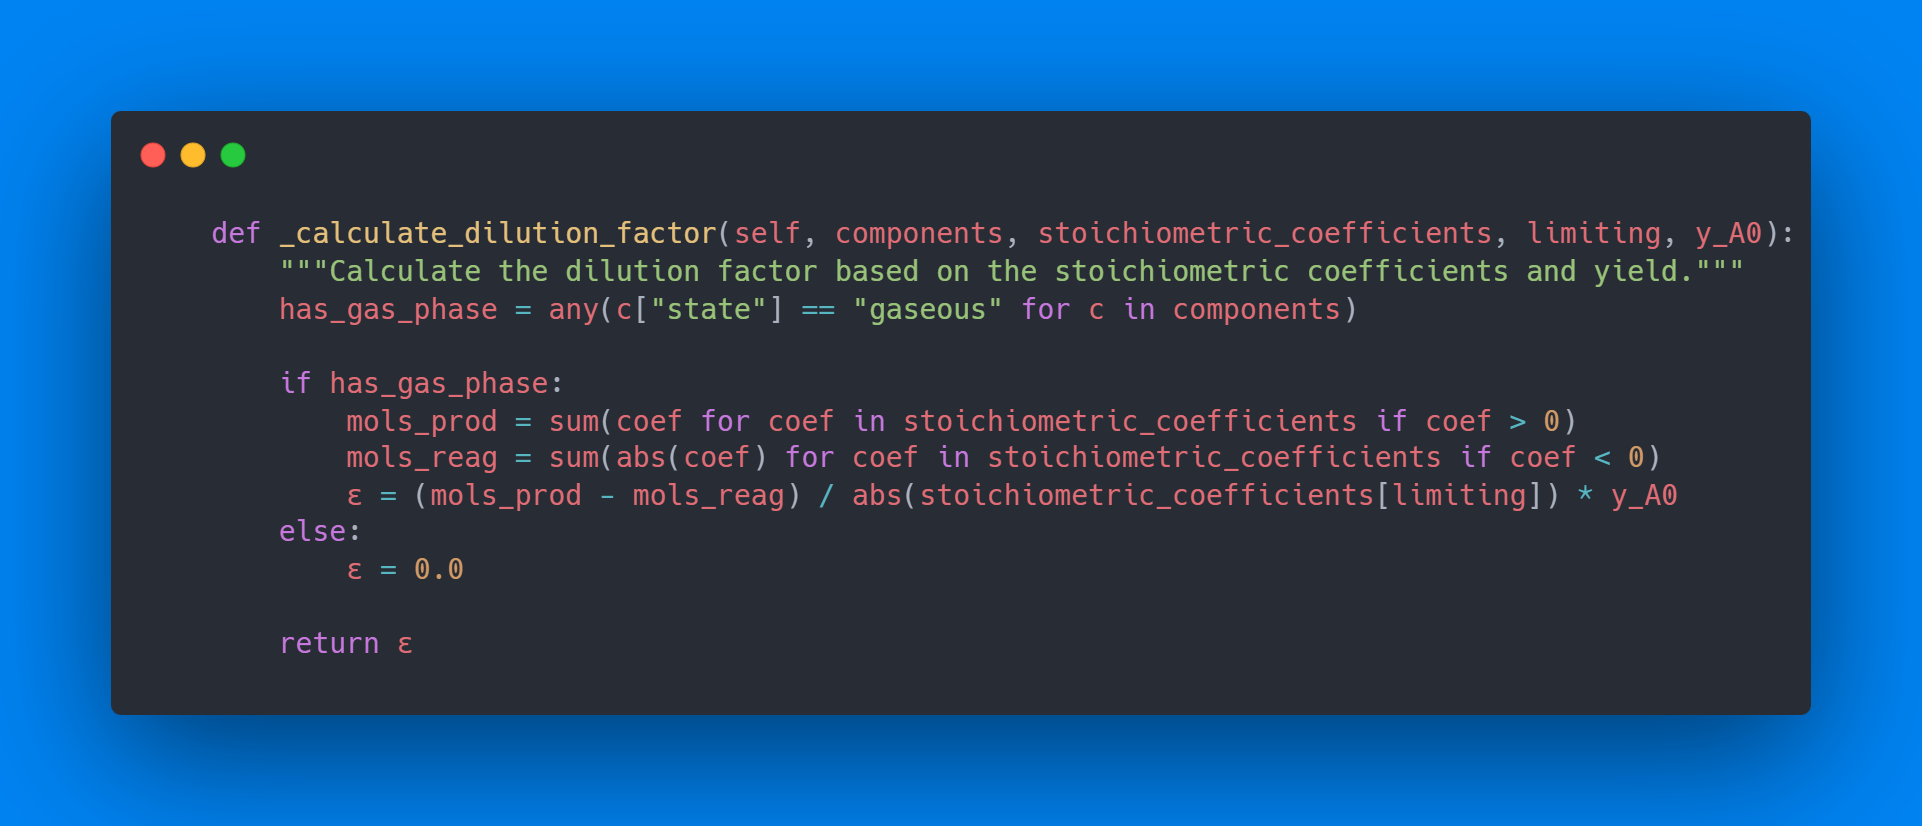
\includegraphics[width=\linewidth]{media/ee059144879c4e4b5d027075171e675a.png}
    \fonte{Autoria própria.}
\end{figure}

Onde $\varepsilon$ representa a variação de número de mols por mol de $A$ reagido. O fator $\psi$ agrega a expansão/contração estequiométrica (via $\varepsilon X$) e as correções de pressão e temperatura em relação às condições iniciais \cite{levenspiel2000}. Essas relações estequiométricas permitem calcular as concentrações de saída de todos os componentes a partir da conversão $X$ do reagente limitante, sendo a base para os balanços nos diferentes modelos de reatores.

\subsubsection{Reator do Tipo CSTR}

O reator do tipo CSTR é um tanque agitado operando em regime contínuo. Assume-se mistura completa no interior do tanque (composição uniforme em todo o volume). A conversão é desenvolvida integralmente dentro do volume do reator, dependendo do balanço entre a cinética de reação e o tempo de residência dos reagentes no tanque.

No sistema implementado, são suportados três casos de uso: (i) conversão desejada e cinética conhecidas (calcula-se o volume do reator necessário), (ii) volume disponível e cinética conhecidas (calcula-se a conversão atingida) e (iii) tempo de residência e cinética conhecidos (calcula-se a conversão atingida). As saídas calculadas pelo algoritmo incluem, entre outros: conversão do reagente limitante $X$, vazão molar do reagente limitante na entrada $F_{A 0}$ vazão volumétrica total na saída $Q_{T}$, volume do reator $V$, taxa de reação $r$ no interior, concentrações de saída $C_{I , s a í d a}$, fator de diluição $\psi$, coeficiente de expansão $\varepsilon$ e tempo de residência $\tau$.

\paragraph{Conversão e Cinética (Cálculo do Volume)}

Passos principais do cálculo:
\begin{itemize}
    \item Identificação do reagente limitante (conforme descrito anteriormente);
    \item Cálculo das vazões molares de entrada pela Equação \ref{eq:molar_flow_in}:
    \begin{equation}
    N_{i 0} = Q_{i} \cdot C_{i 0 e}
    \label{eq:molar_flow_in}
    \end{equation}
    para cada componente, bem como da vazão volumétrica total pela Equação \ref{eq:total_flow}:
    \begin{equation}
    Q_{T} = \sum_{}^{} Q_{i}
    \label{eq:total_flow}
    \end{equation}
    As concentrações iniciais (após mistura das correntes de alimentação) são dadas pela Equação \ref{eq:initial_conc}:
    \begin{equation}
    C_{i 0} = \frac{N_{i 0}}{Q_{T}}
    \label{eq:initial_conc}
    \end{equation}
    \item Cálculo do fator de diluição total $\psi$ com a conversão alvo $X$ (Equação \ref{eq:dilution_factor});
    \item Cálculo da taxa de reação $r$ a partir da constante cinética $k$ e das concentrações na saída (considerando $X$), supondo regime isotérmico \cite{fogler2009};
    \item Aplicação do balanço no CSTR para o reagente limitante.
\end{itemize}

Para conversão $X$ conhecida, a equação de \textit{design} é dada por:

\begin{equation}
V = \frac{F_{A 0} \cdot X}{- r_{A}}
\label{eq:cstr_design}
\end{equation}

Dos quais,
\begin{itemize}
    \item $F_{A 0}$ – Vazão molar de $A$ na entrada
    \item $r$ - Taxa de consumo de $A$ por unidade de volume no interior do reator
\end{itemize}

Cálculo do tempo de residência:

\begin{equation}
\tau = \frac{Q_{T}}{V}
\label{eq:residence_time}
\end{equation}

\begin{figure}[H]
    \centering
    \caption{Código da função \textit{\_conversion\_and\_kinetics\_in\_cstr()} – Parte 1/2}
    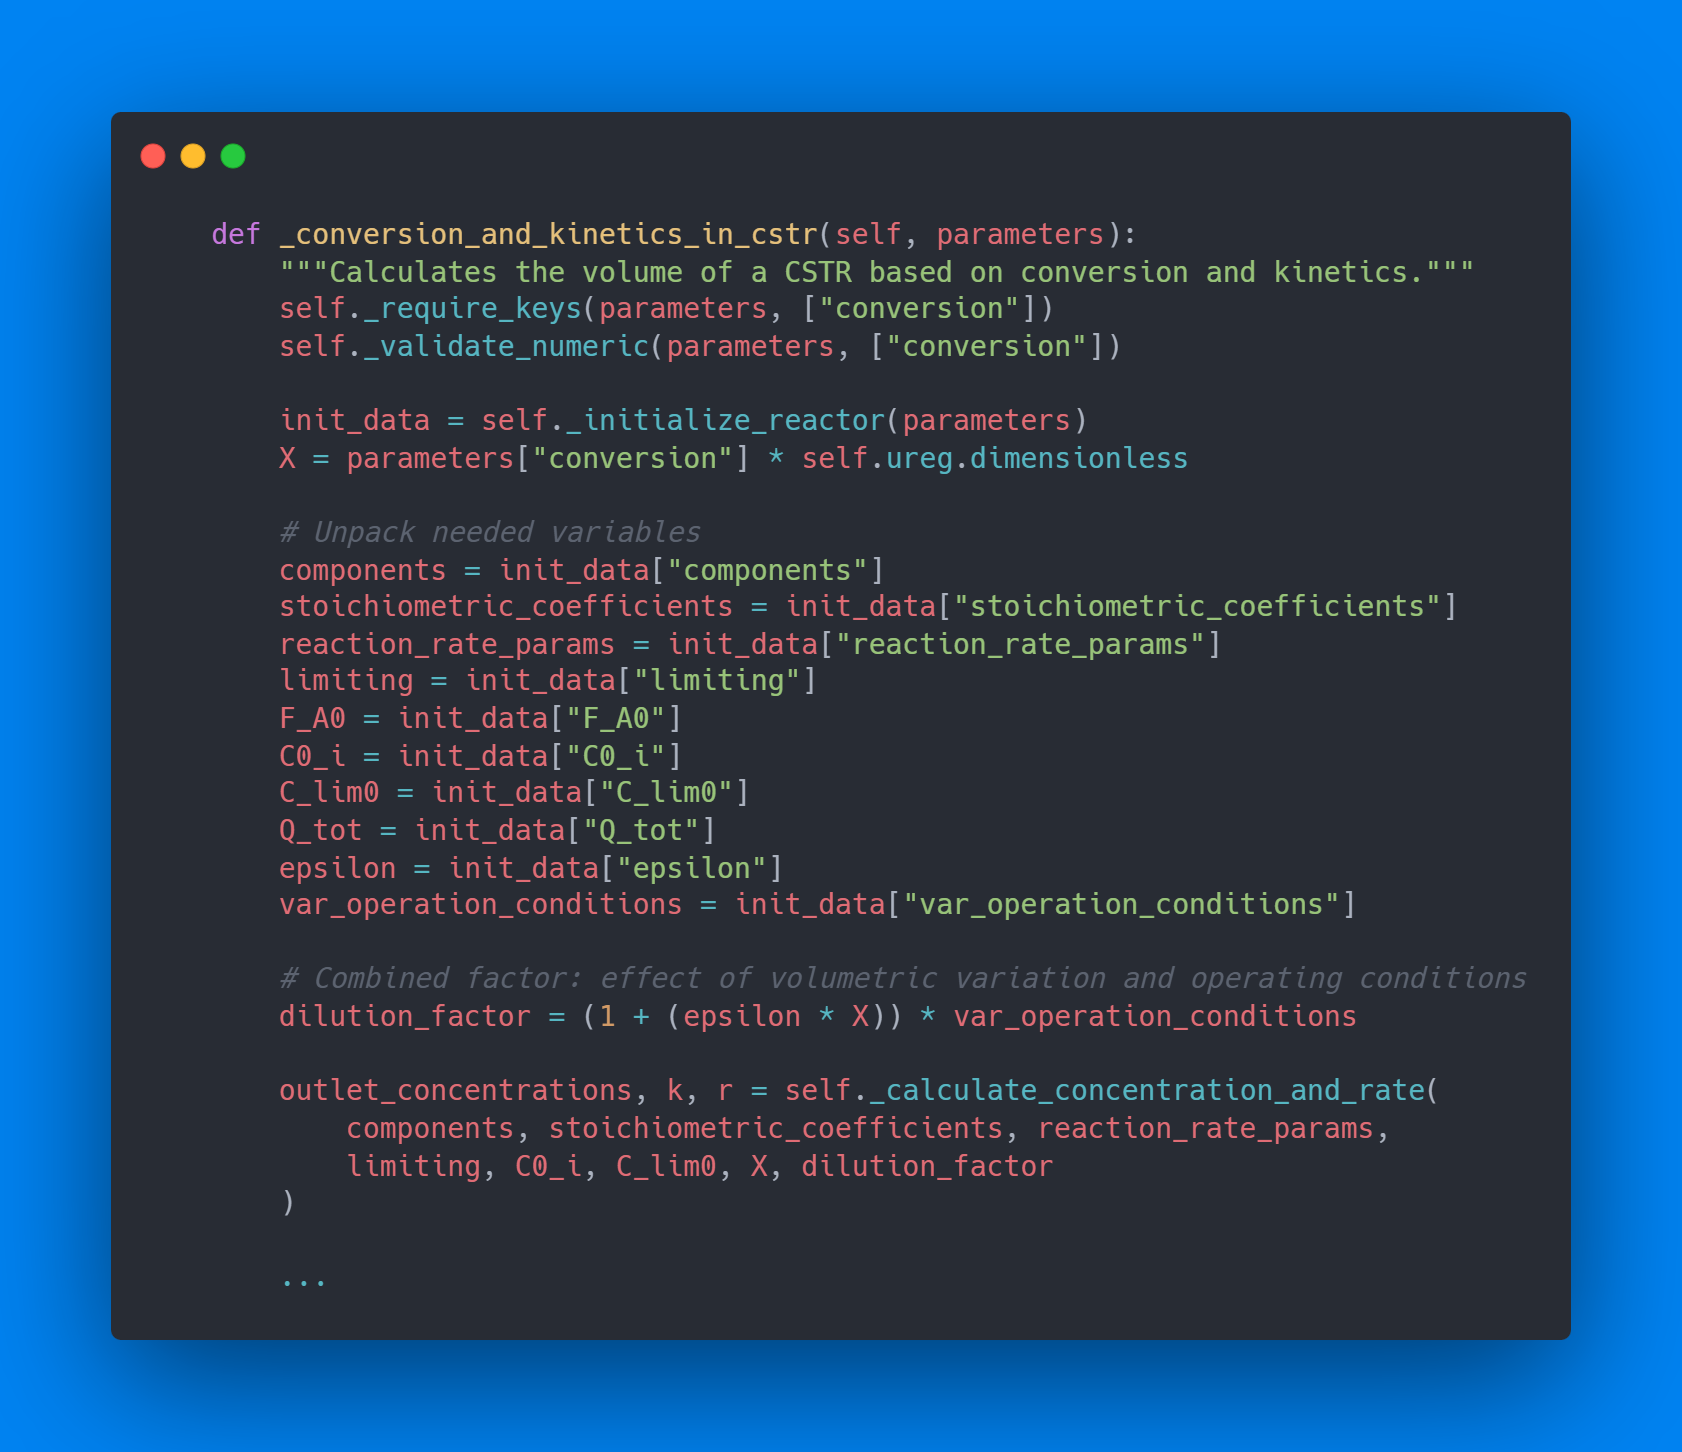
\includegraphics[width=\linewidth]{media/aa91328cd1e15918342126f874911bd1.png}
    \fonte{Autoria própria.}
\end{figure}

\begin{figure}[H]
    \centering
    \caption{Código da função \textit{\_conversion\_and\_kinetics\_in\_cstr()} – Parte 2/2}
    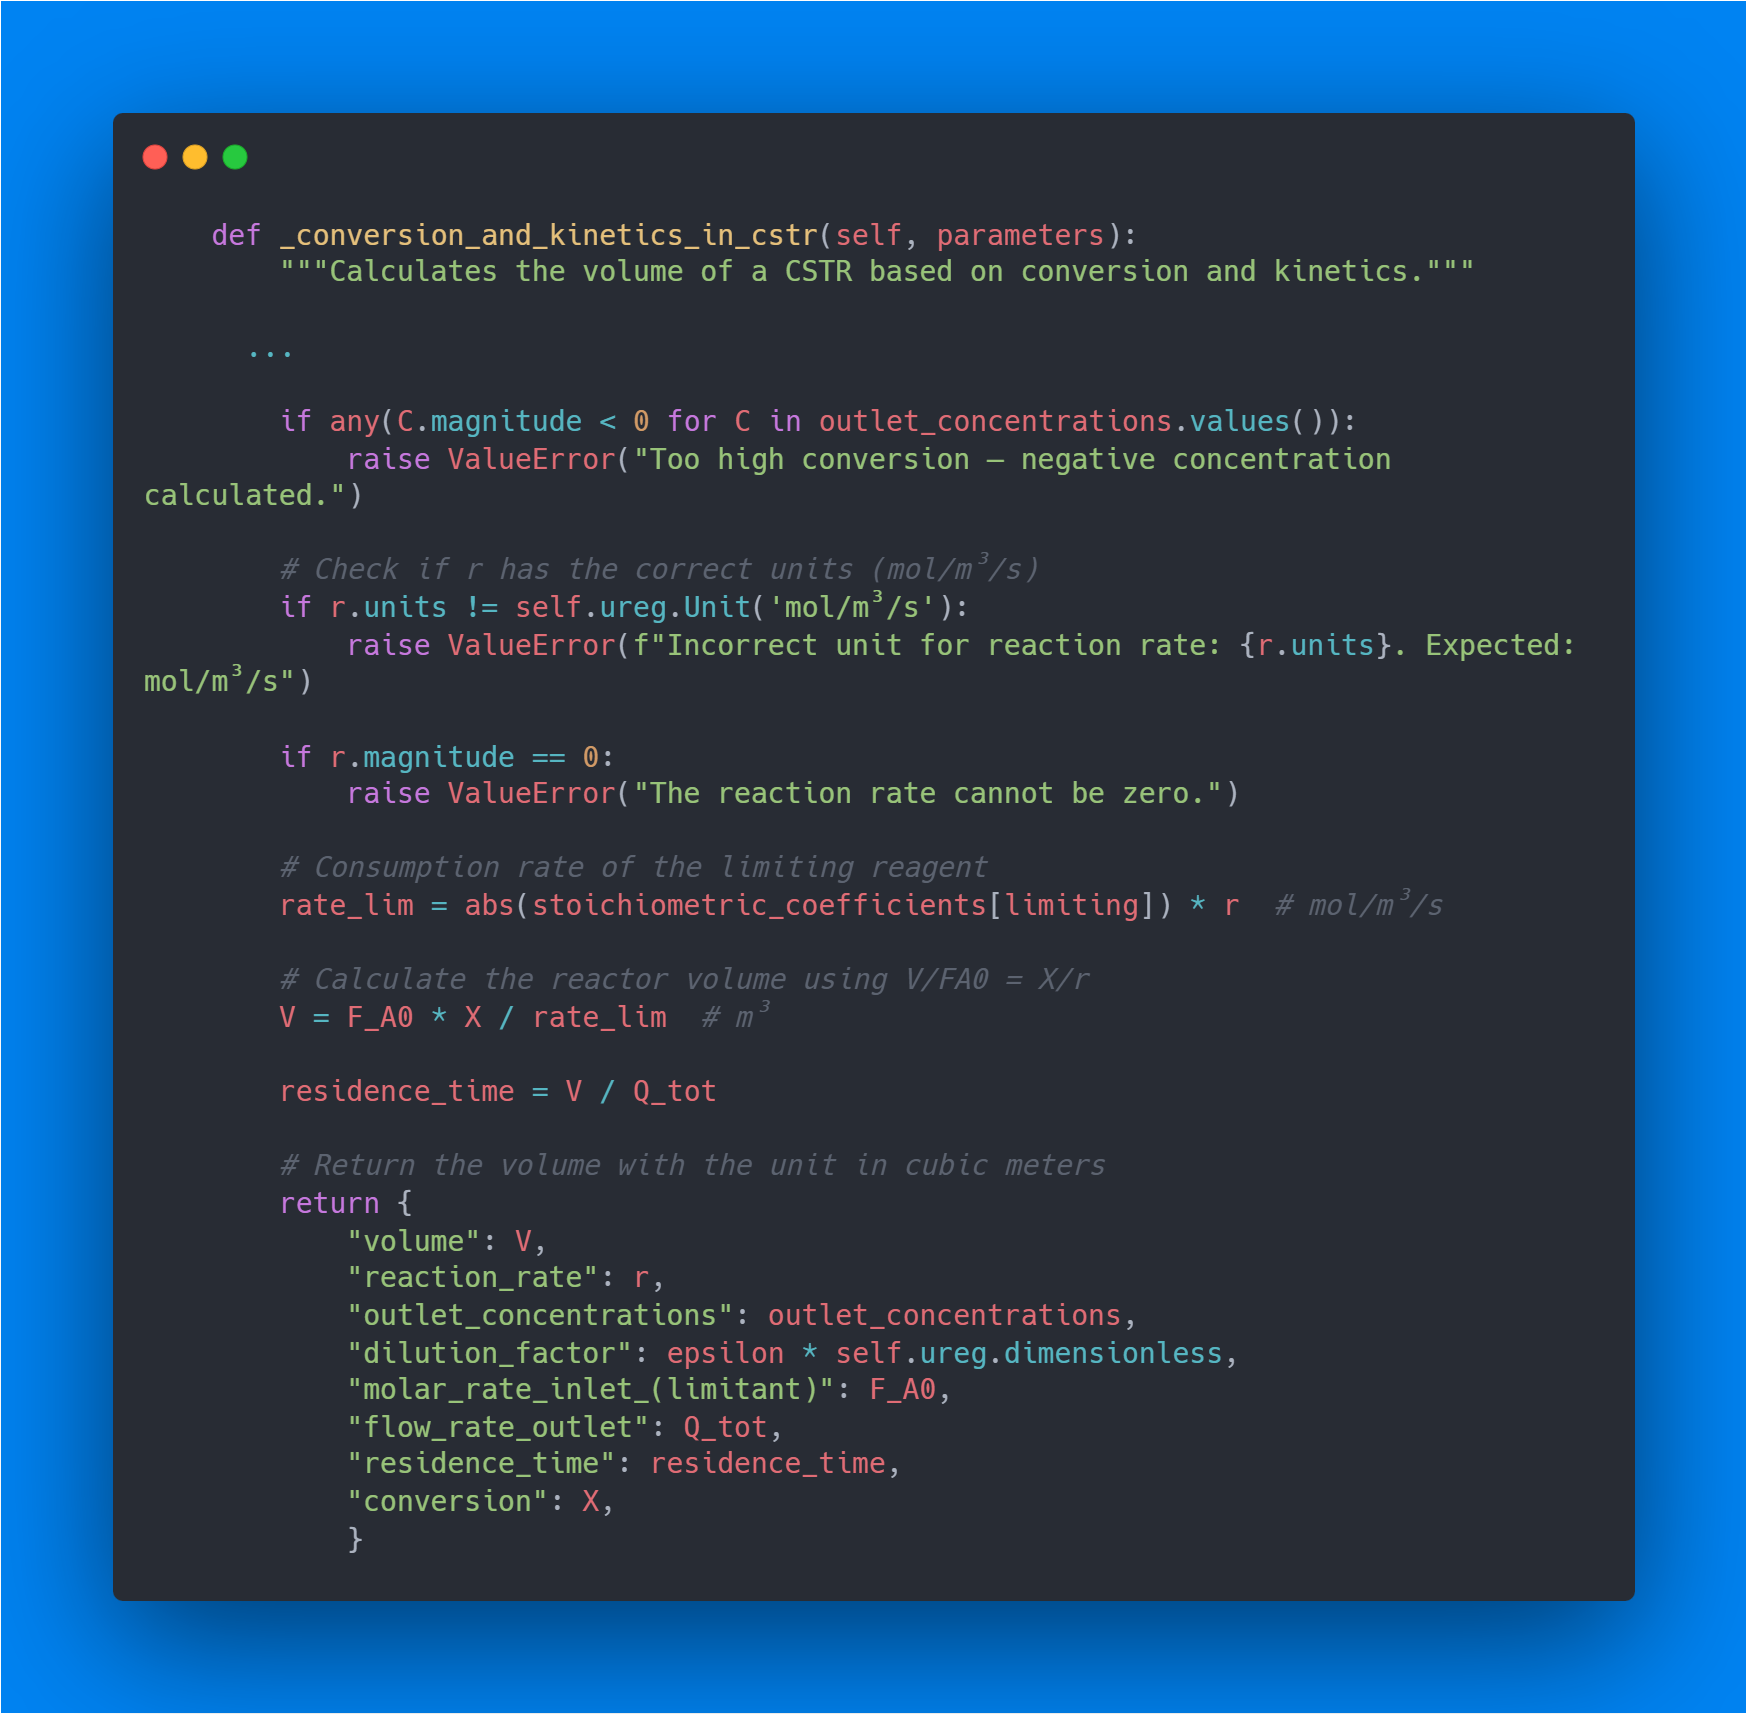
\includegraphics[width=\linewidth]{media/f0bdf786918c58bf0ba1a79c0722c17c.png}
    \fonte{Autoria própria.}
\end{figure}

A fim de simplificar as lógicas, é usada a função \textit{\_initialize\_reactor(),} que calcula as concentrações e vazões de cada componente na entrada, assim como o \textit{épsilon,} fator de diluição, temperaturas e pressões iniciais e finais e o reagente limitante.

\begin{figure}[H]
    \centering
    \caption{Código da função \textit{\_initialize\_reactor()} – Parte 1/2}
    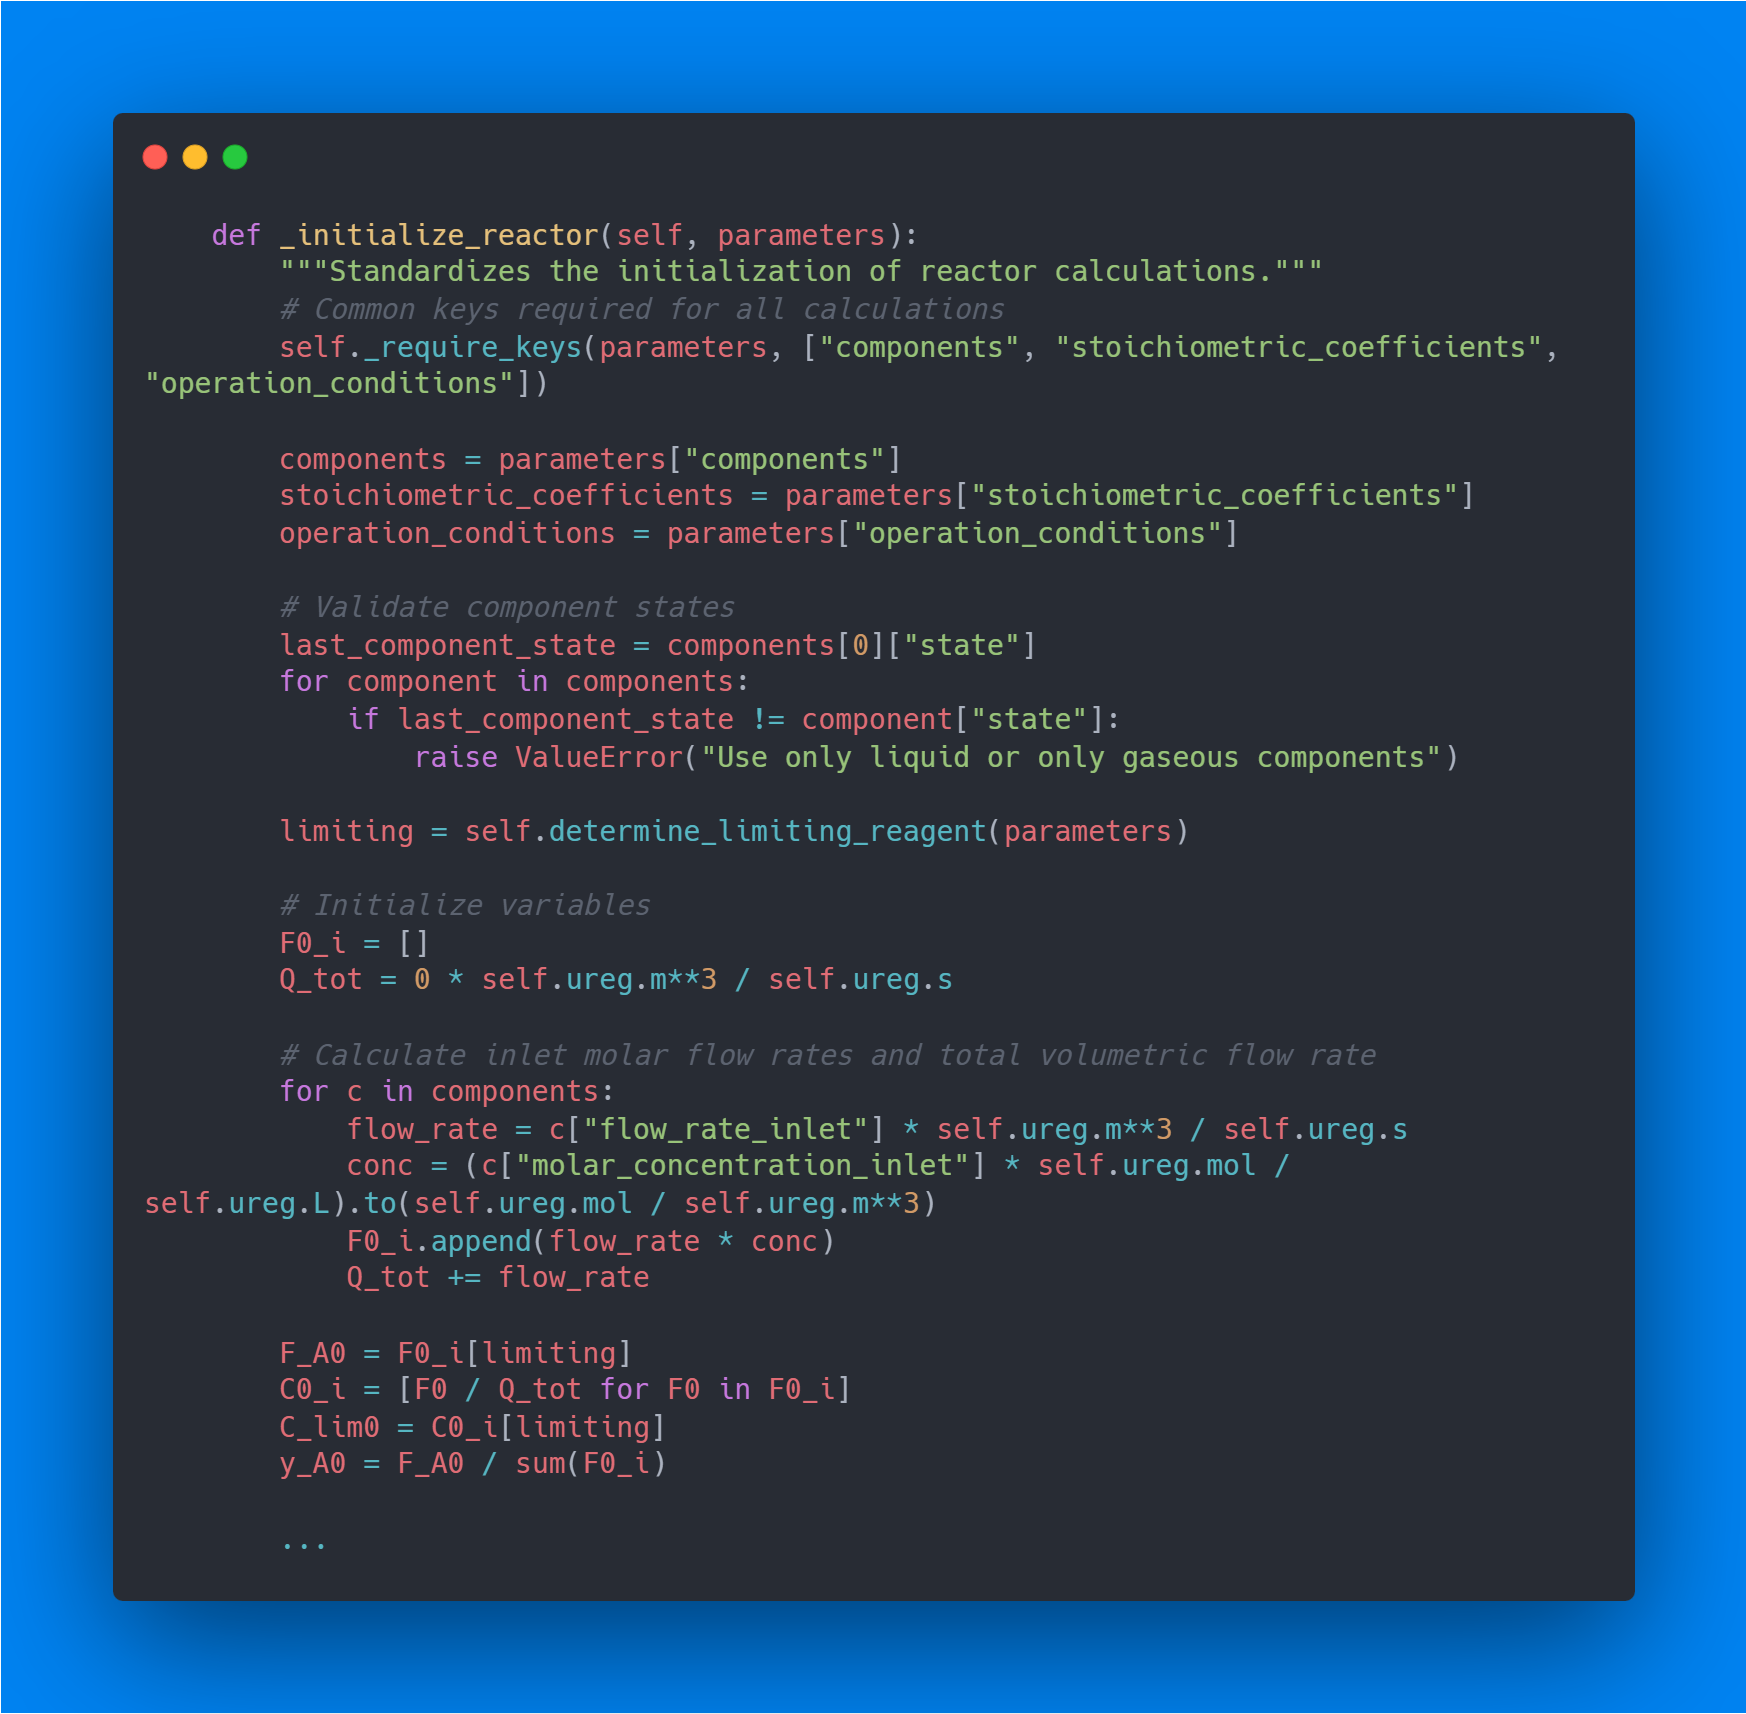
\includegraphics[width=\linewidth]{media/485e4ad0e02b6938ff532098fa54ad4f.png}
    \fonte{Autoria própria.}
\end{figure}

\begin{figure}[H]
    \centering
    \caption{Código da função \textit{\_initialize\_reactor()} – Parte 2/2}
    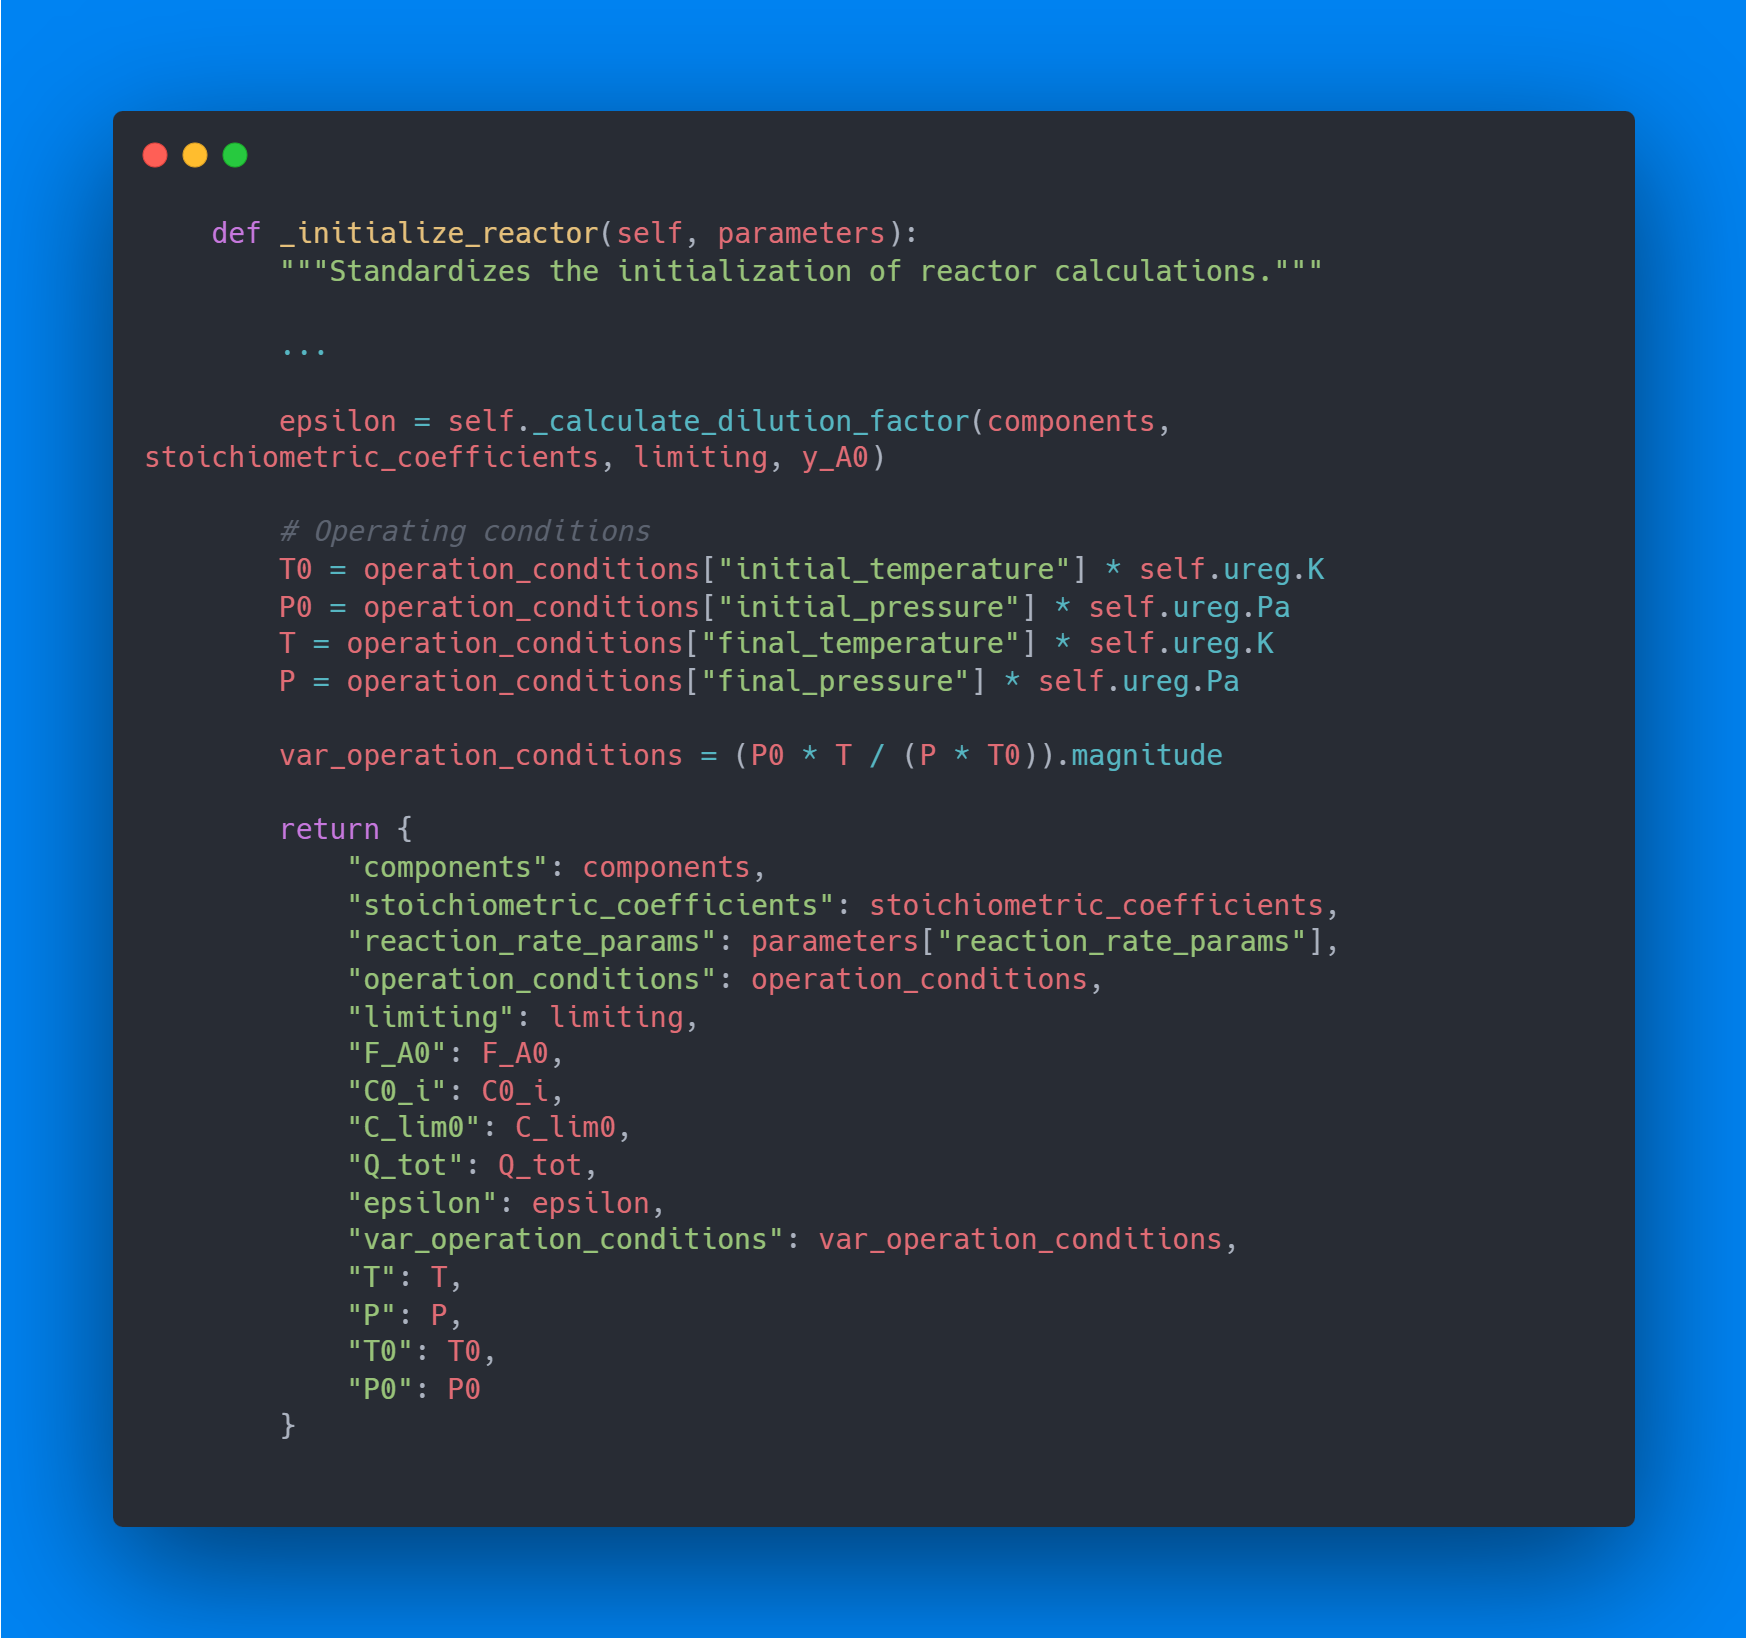
\includegraphics[width=\linewidth]{media/b4897428706f25f6e44b384b57872fd6.png}
    \fonte{Autoria própria.}
\end{figure}

\paragraph{Volume e Cinética (Cálculo da Conversão)}

Nesse caso, são conhecidos o volume do reator $V$ e a cinética (expressão da taxa $r ( C_{i} )$, incluindo $k$). Deseja-se determinar a conversão $X$ atingida no CSTR. Isolando $X$ na equação de \textit{design} do CSTR obtém-se uma equação implícita. Define-se então uma função objetivo:

\begin{equation}
f ( x ) = \frac{{| v}_{A} | \cdot r_{A} \cdot V}{F_{A 0}} - X
\label{eq:cstr_obj_function}
\end{equation}

Então encontra-se sua raiz na faixa 0<X<1, tipicamente utilizando o método de Brent, dada a monotonicidade esperada de $f ( x )$. A raiz X que satisfaz $f ( x ) = 0$ corresponde à conversão no reator.

\begin{figure}[H]
    \centering
    \caption{Código da função \textit{\_volume\_and\_kinetics\_in\_cstr()} – Parte 1/2}
    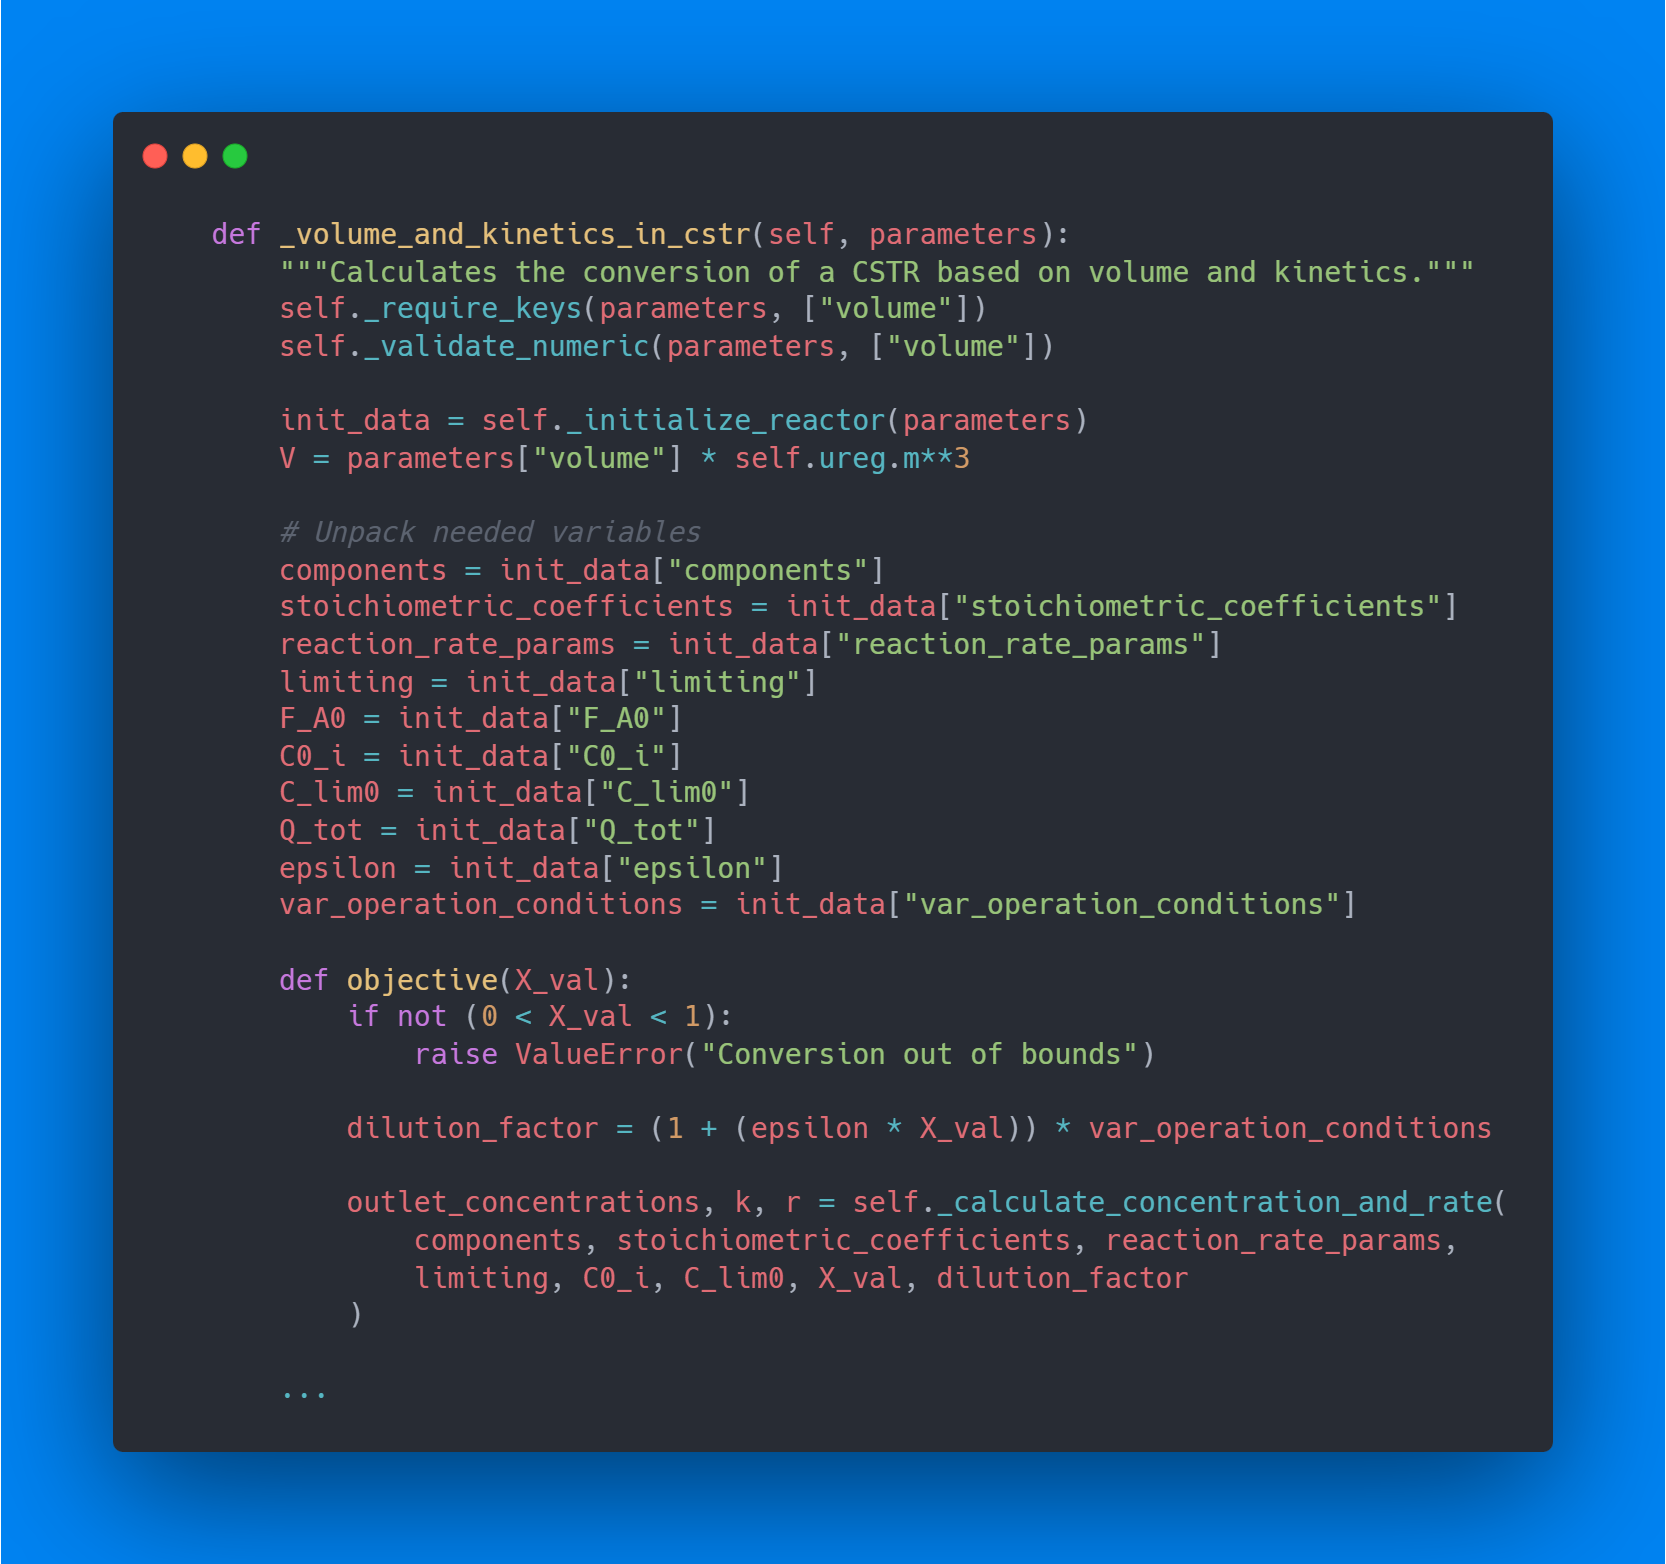
\includegraphics[width=\linewidth]{media/0f165d3bd542e0d3d61acb8052eccbe8.png}
    \fonte{Autoria própria.}
\end{figure}

\begin{figure}[H]
    \centering
    \caption{Código da função \textit{\_volume\_and\_kinetics\_in\_cstr()} – Parte 2/2}
    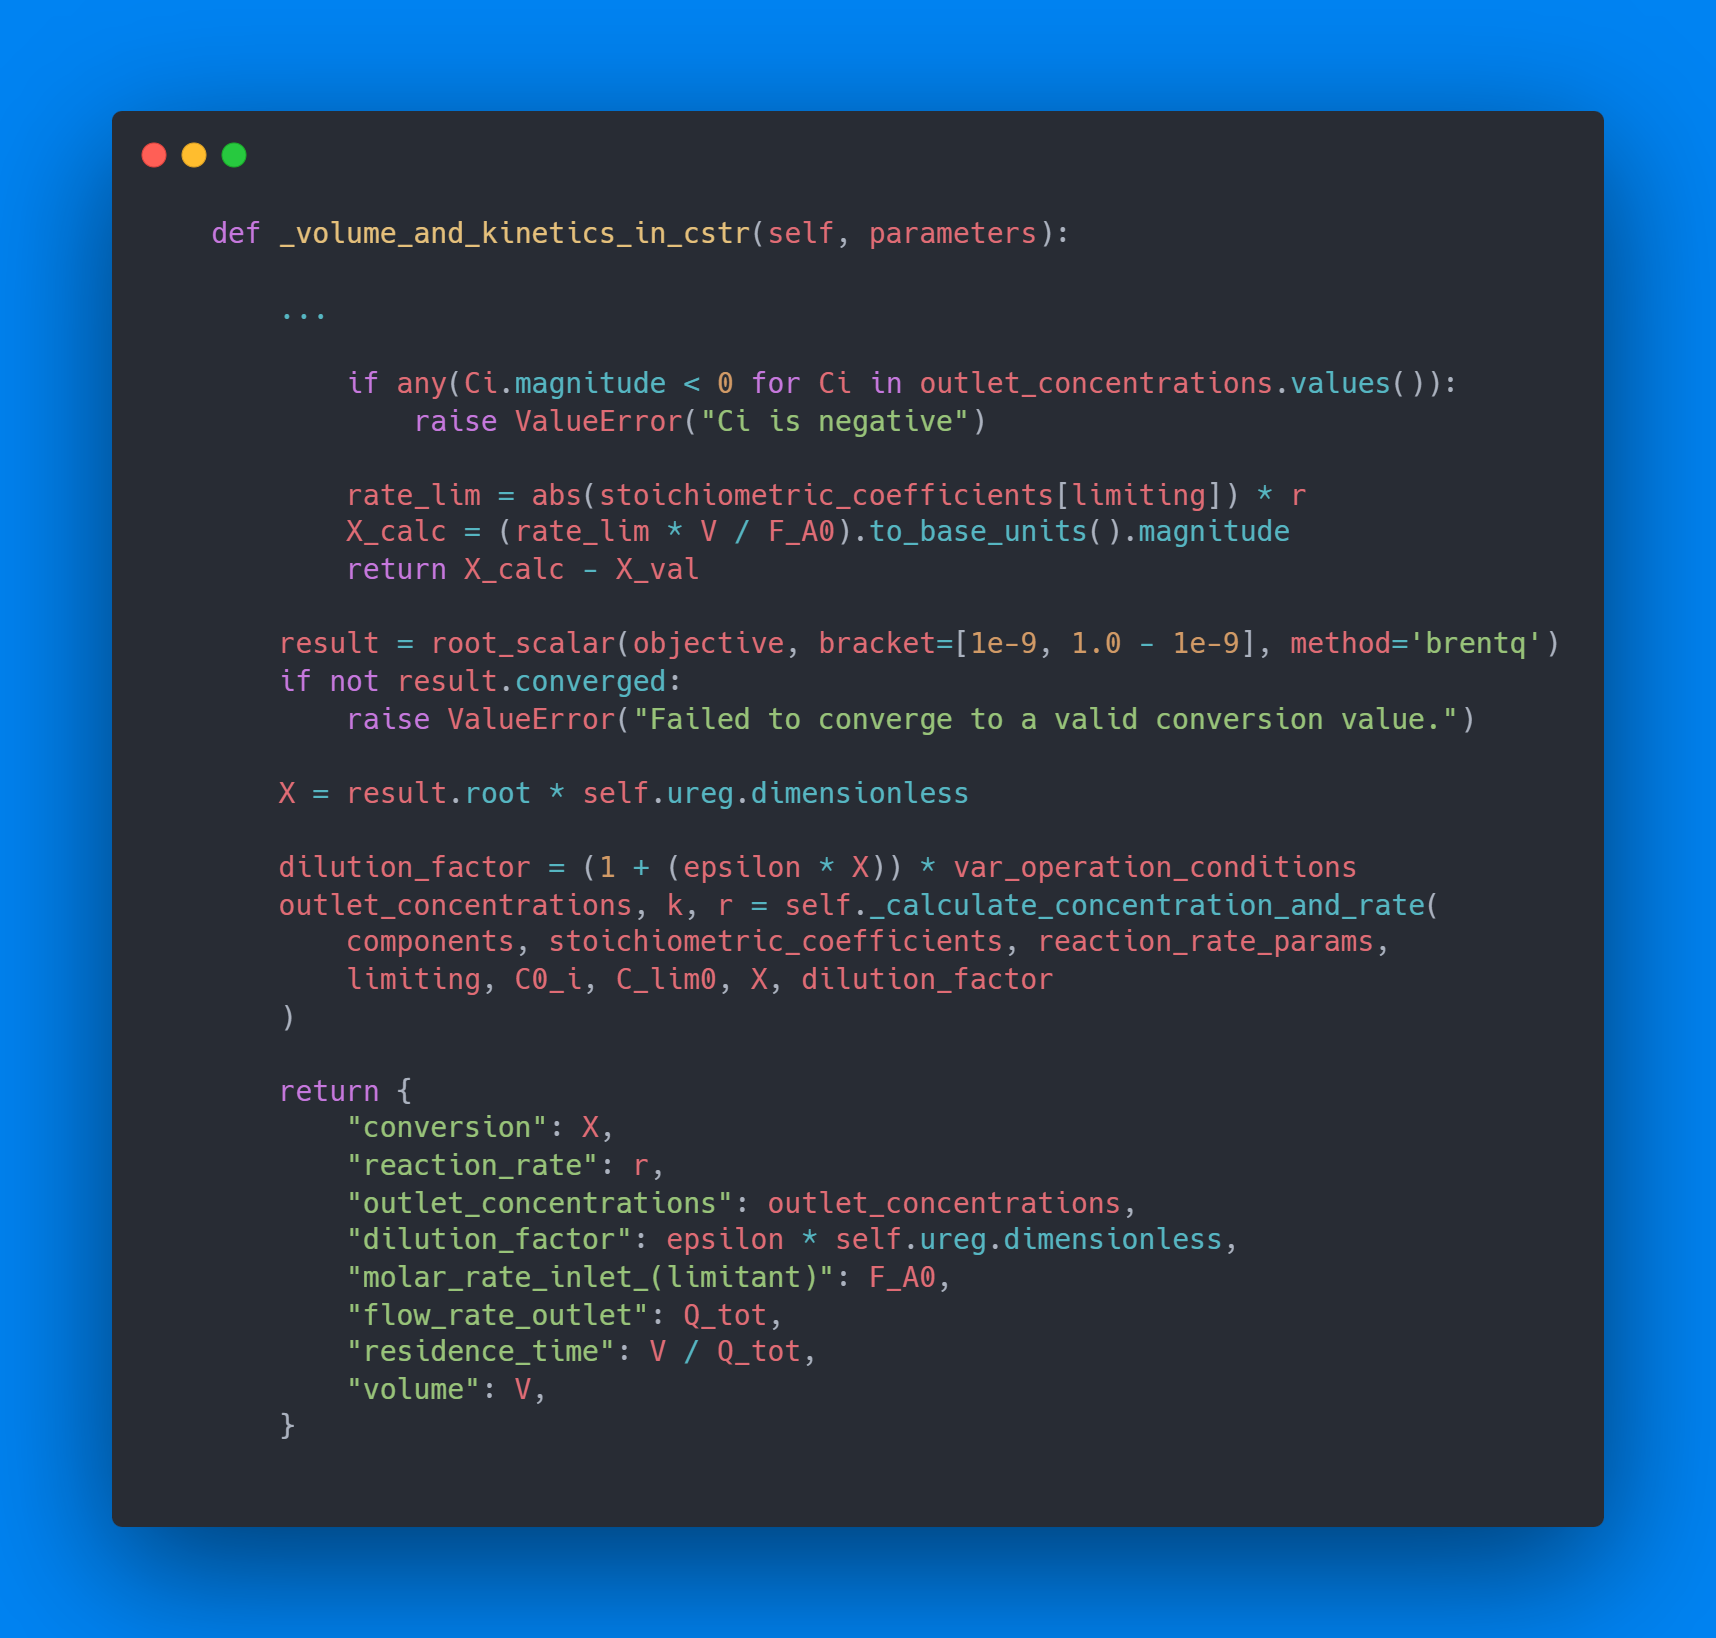
\includegraphics[width=\linewidth]{media/7ec6ccfb51ad2af7ea36f138d95073f2.png}
    \fonte{Autoria própria.}
\end{figure}

\paragraph{Tempo de Residência e Cinética}

Conhecido o tempo de residência $\tau$, calcula-se inicialmente pela Equação \ref{eq:volume_calc}:
\begin{equation}
V = Q_{T} \cdot \tau
\label{eq:volume_calc}
\end{equation}
Em seguida, o problema se reduz ao caso anterior: aplica-se a mesma função objetivo $f ( X )$ da Equação \ref{eq:cstr_obj_function} e resolve-se numericamente para $X$, obtendo a conversão atingida no CSTR com tempo de residência $\tau$ especificado.

\begin{figure}[H]
    \centering
    \caption{Código da função \textit{\_residence\_time\_and\_kinetics\_in\_cstr()} – Parte 1/2}
    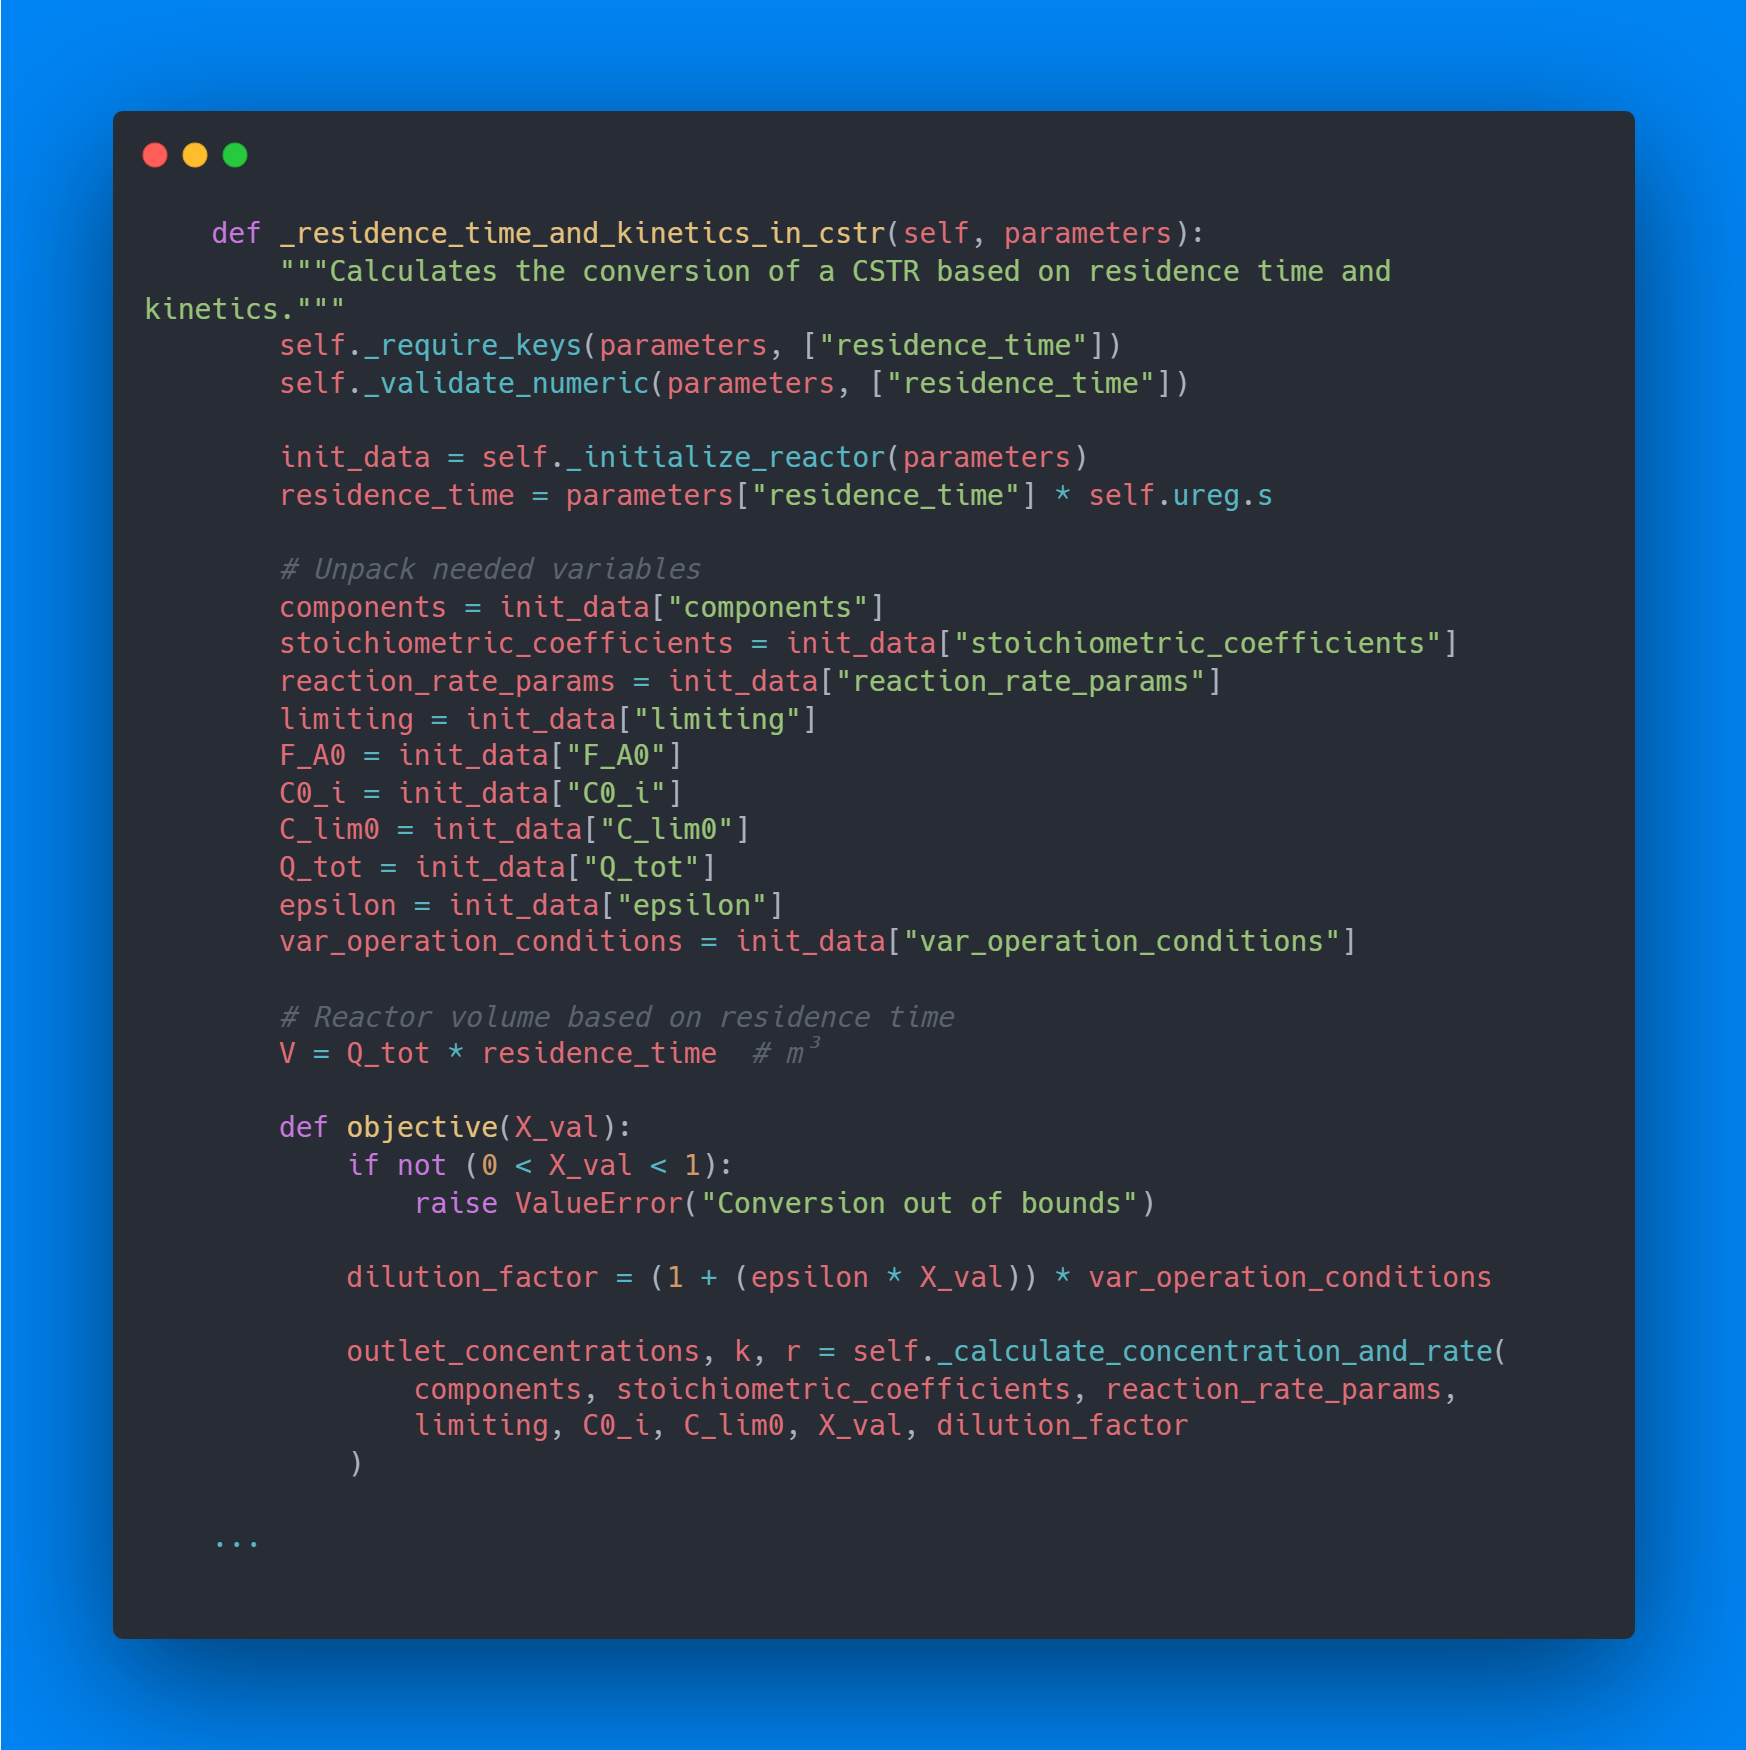
\includegraphics[width=\linewidth]{media/a4e6fbc1e6e830fc59e501c16af6375b.png}
    \fonte{Autoria própria.}
\end{figure}

\begin{figure}[H]
    \centering
    \caption{Código da função \textit{\_residence\_time\_and\_kinetics\_in\_cstr()} – Parte 2/2}
    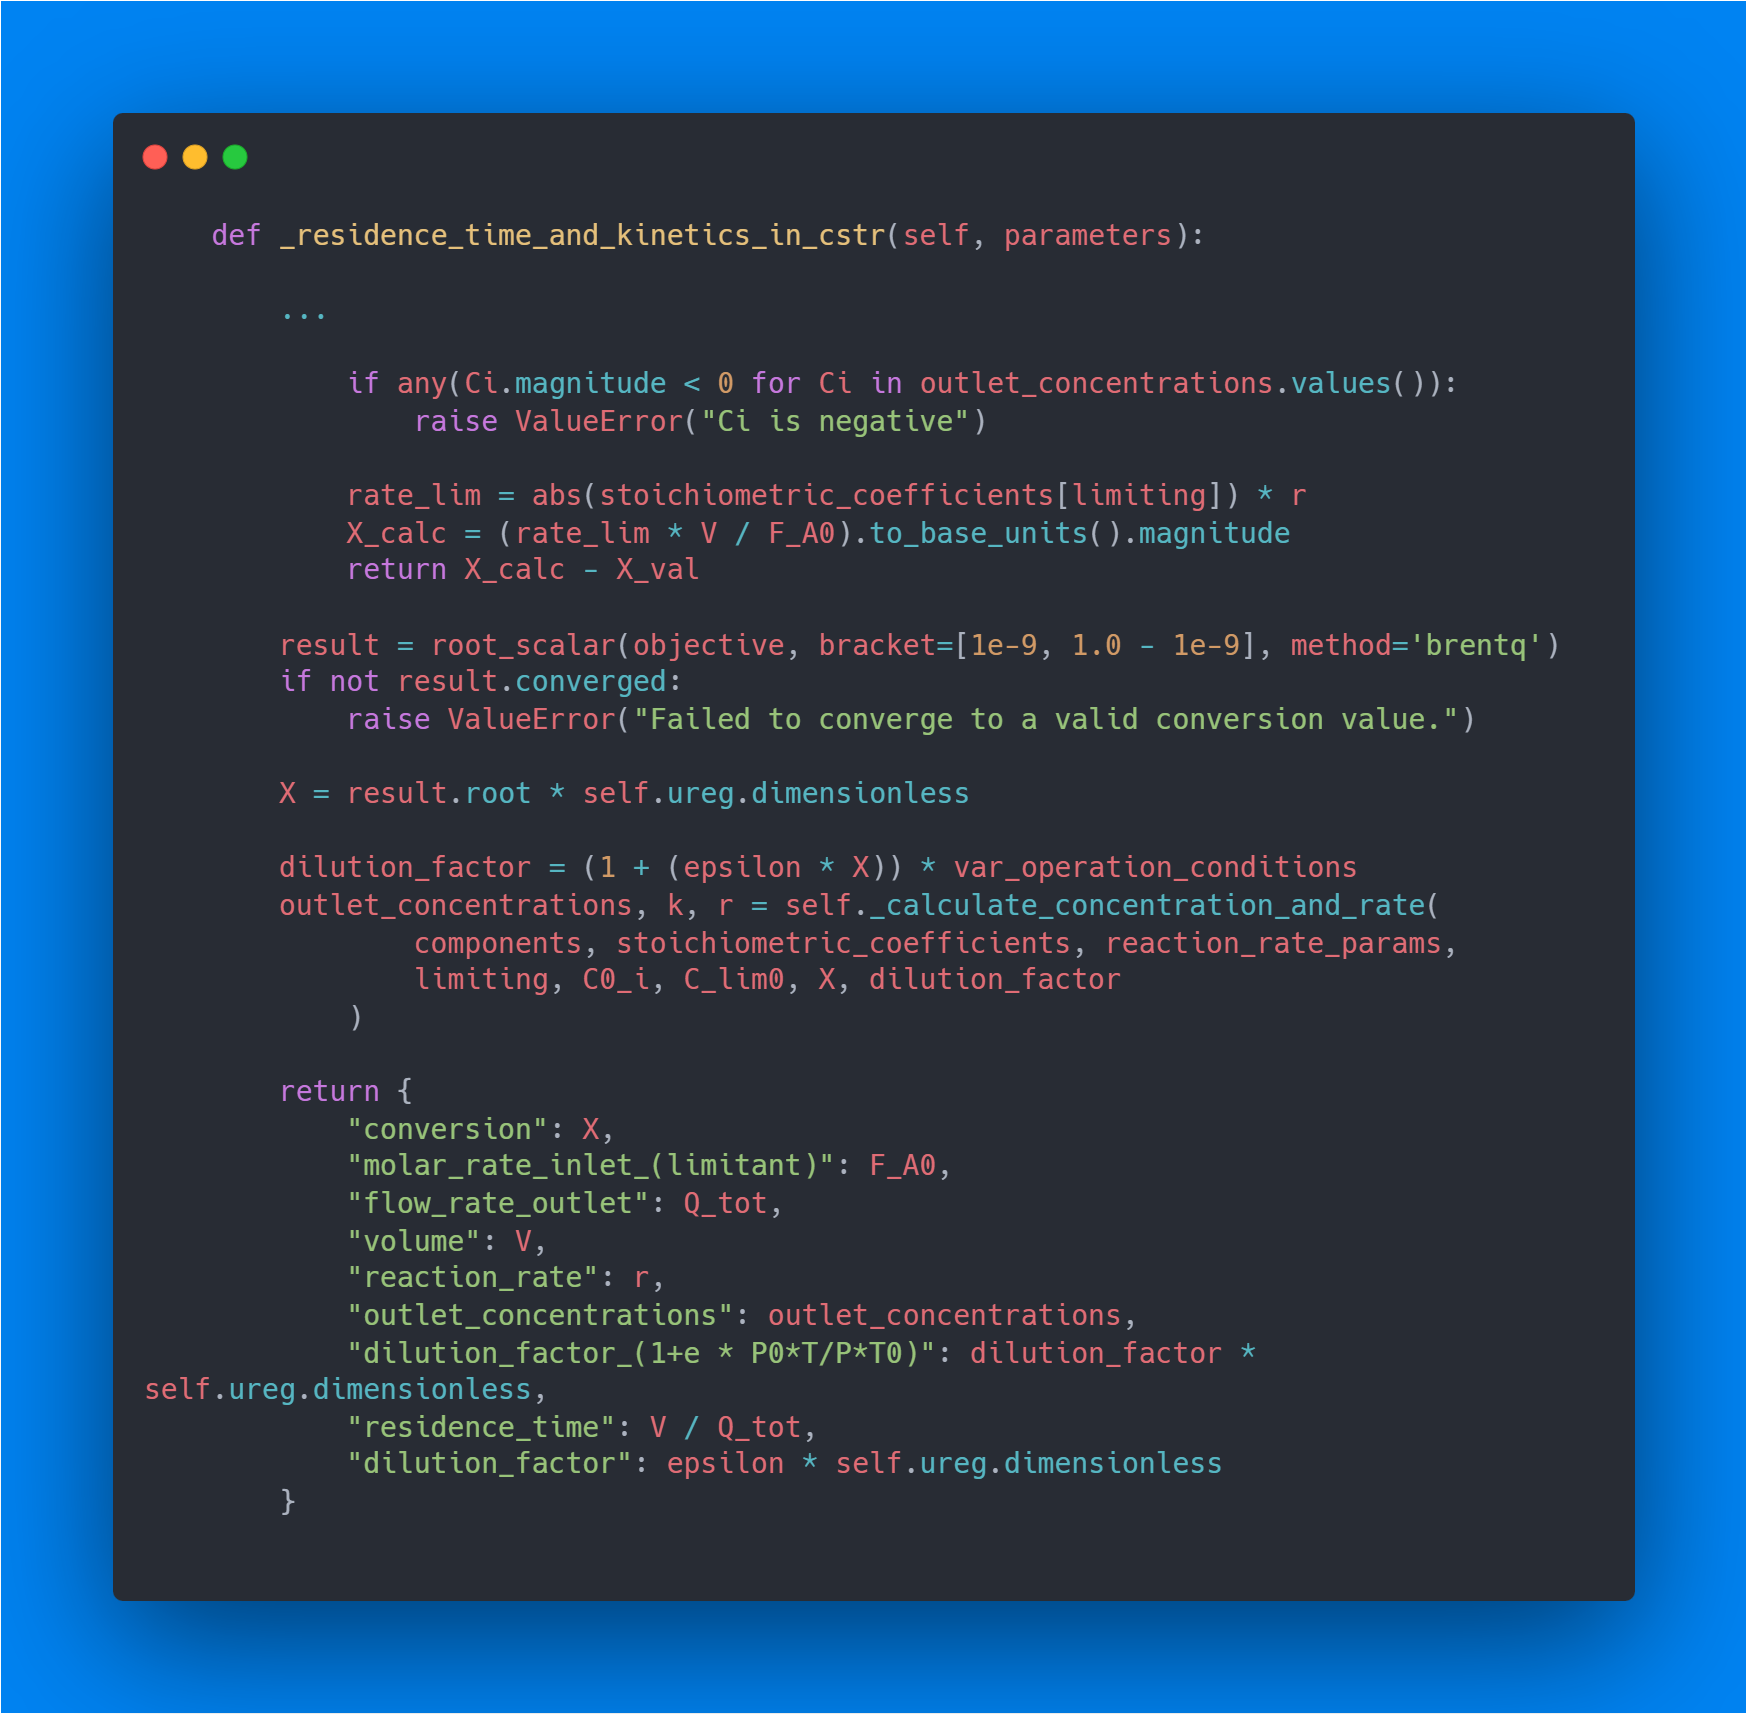
\includegraphics[width=\linewidth]{media/1b0f58c8b9359a99c0550e6a7c4d13f7.png}
    \fonte{Autoria própria.}
\end{figure}
